% Ingeniería de Requerimientos
% Este archivo se incluye desde main.tex con \input.
\section{Ingeniería de Requerimientos}
\subsection{Introducción del Capítulo}
En el presente capítulo se aborda la fase de Ingeniería de Requerimientos, un paso fundamental para traducir las necesidades de los atletas híbridos en especificaciones técnicas claras y medibles. A partir del análisis metodológico y de las alternativas evaluadas previamente, aquí se define el comportamiento esperado del sistema, la interacción de sus procesos principales y las restricciones bajo las cuales debe operar. En primer lugar, se presentará el Modelo de Negocios enfocado en los procesos operativos core de la plataforma, seguido por el modelo detallado de requerimientos funcionales y no funcionales, para finalmente establecer los Casos de Uso que guiarán la construcción de la arquitectura de software.

\subsection{Modelo de Negocios (Procesos Core)}
En este capítulo, el modelo de negocios no se refiere a cómo gana dinero el proyecto, porque eso ya se analizó en la factibilidad económica del capítulo anterior. Aquí se refiere a los procesos principales que entregan valor al atleta. Se describen cinco procesos, y entre ellos cubren el registro de fuerza, de cardio y de comidas, el cruce de datos, la red social y el plan sugerido.
\\\\
Los procesos se dibujan con carriles, al estilo de BPMN (Business Process Model and Notation). Cada carril representa a un participante, el círculo simple marca el inicio, el círculo doble marca el fin y los rombos marcan las decisiones. Las tareas están numeradas, y después de cada diagrama se explica qué ocurre en cada una.
\newpage
\subsubsection{Proceso 1: Registro de Cardio y Cálculo de Fatiga Cruzada}
Este proceso muestra cómo una sesión de cardio entra a la aplicación, venga de donde venga, y cómo se cruza con el resto de los datos para avisar al atleta si está acumulando demasiada fatiga. Los participantes son el atleta, la aplicación y el reloj junto con la app de salud del teléfono. Responde a los requerimientos R02 y R03.

\begin{figure}[h!]
    \centering
    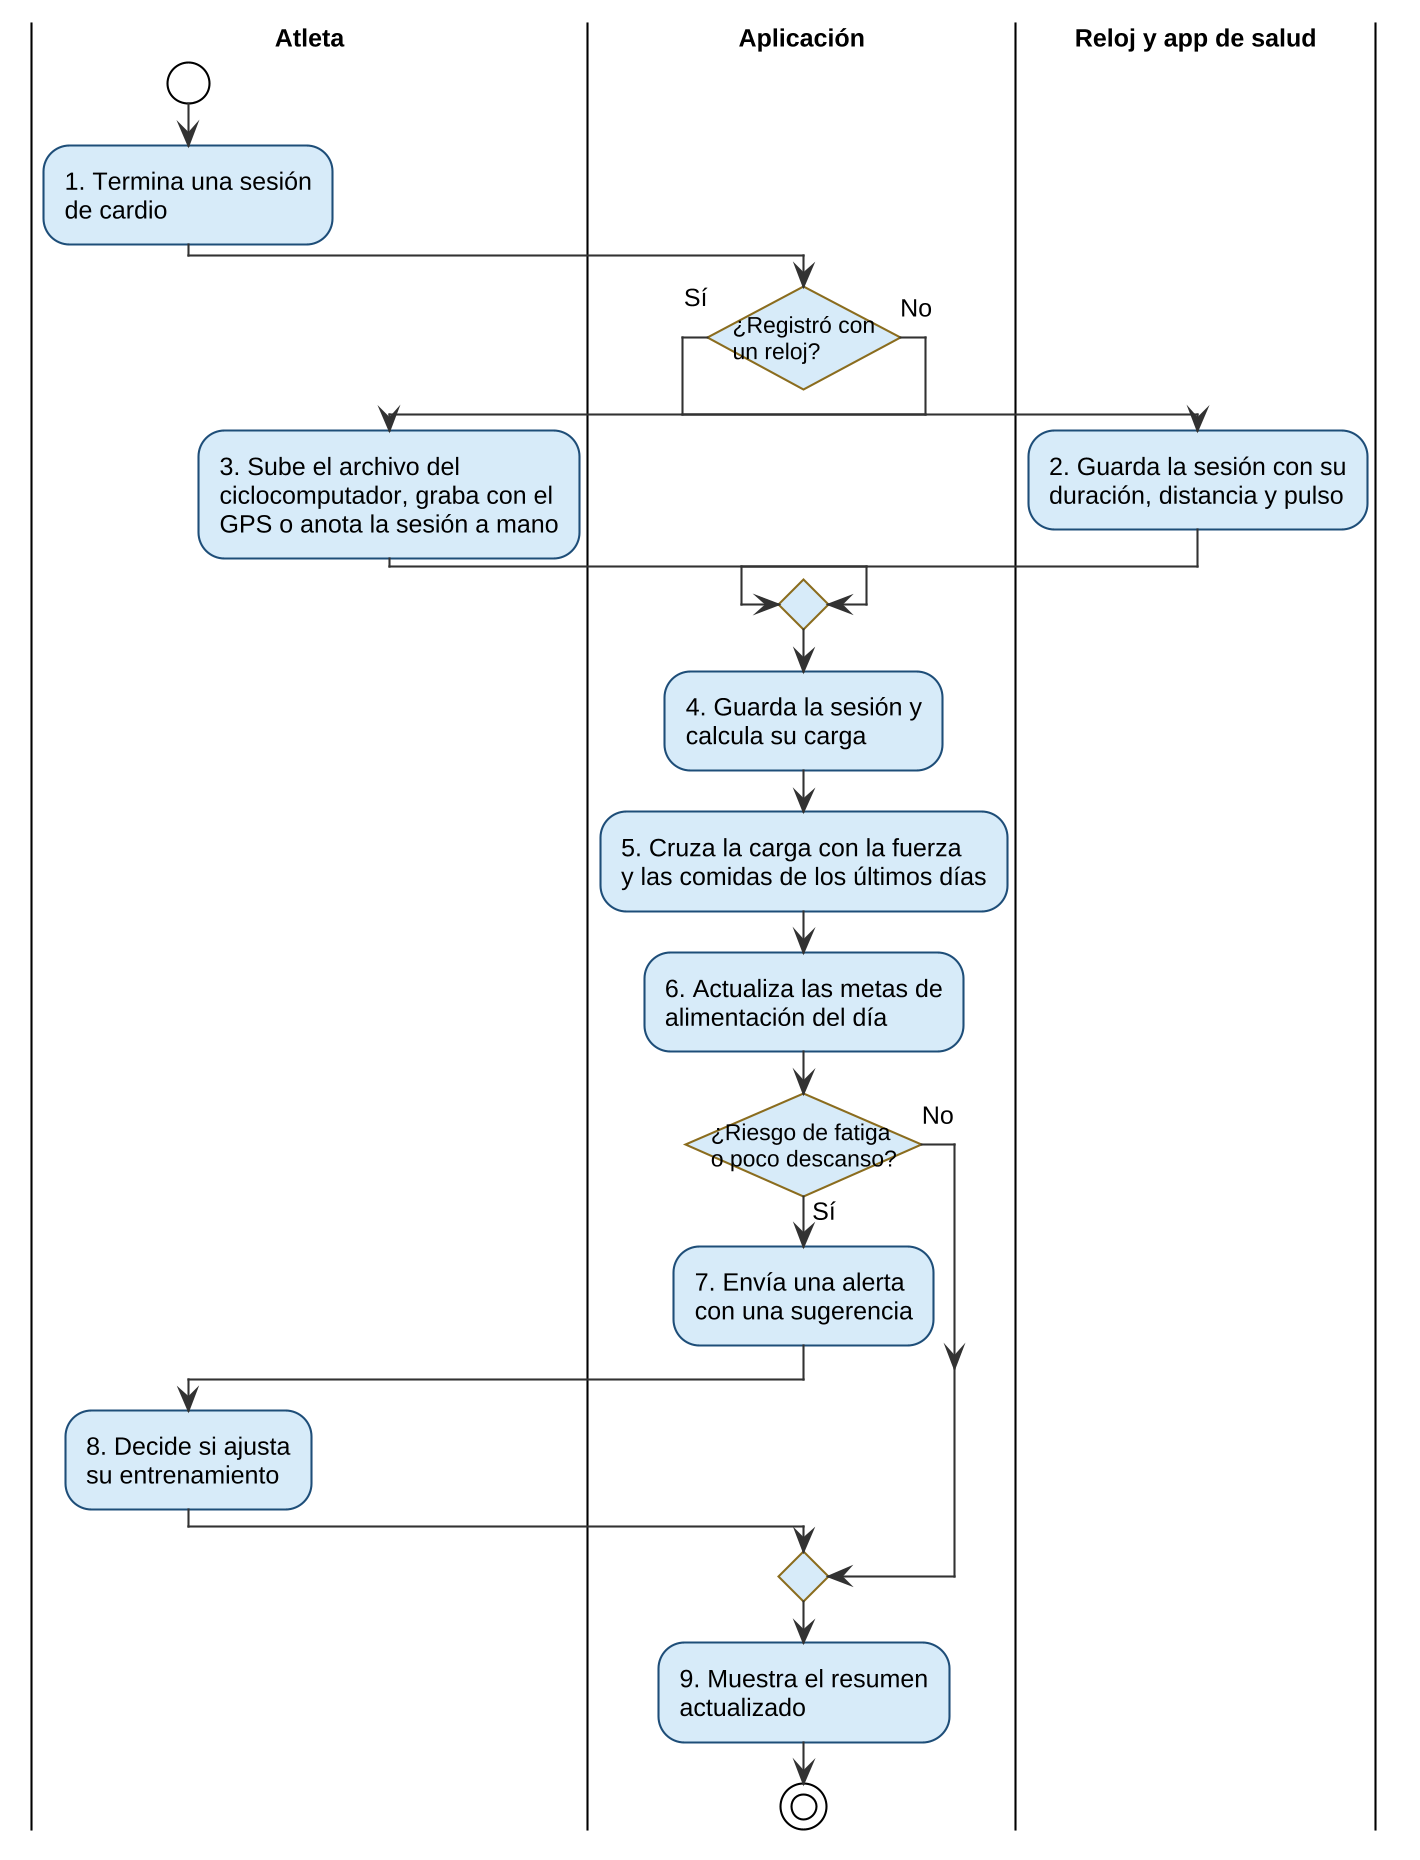
\includegraphics[width=0.68\textwidth]{figuras/procesos/bpmn_proceso1.png}
    \caption{Proceso 1: Registro de cardio y cálculo de fatiga cruzada.}
    \label{fig:bpmn_fatiga}
\end{figure}
\newpage
\textbf{Tareas del proceso}

\begin{enumerate}
    \item \textbf{Termina una sesión de cardio:} El proceso parte cuando el atleta termina una salida de ciclismo, running o trekking.
    \item \textbf{Guarda la sesión:} Si entrenó con un reloj, este guarda la sesión en Health Connect o Apple Salud. La aplicación la trae sola, siempre que el atleta haya dado permiso para leer esos datos.
    \item \textbf{Sube el archivo, graba o anota:} Si no usó un reloj, el atleta tiene tres opciones. Puede subir el archivo \texttt{.fit} de su ciclocomputador, grabar la ruta con el GPS del teléfono o anotar la sesión a mano. En las dos últimas también indica qué tan duro la sintió (RPE).
    \item \textbf{Guarda la sesión y calcula su carga:} La carga se calcula según la disciplina y los datos disponibles, como la potencia en ciclismo, el ritmo en running y el desnivel en trekking. Si faltan esos datos, se usan el pulso o el RPE. Si la misma sesión llega por dos vías, se usa la que tiene más detalle.
    \item \textbf{Cruza la carga:} La aplicación junta esta carga con las sesiones de fuerza y las comidas de los últimos días para estimar la fatiga cruzada. También revisa cuánto tiempo pasó entre sesiones de distinto tipo.
    \item \textbf{Actualiza las metas de alimentación:} Las metas del día cambian según lo entrenado, por ejemplo con más carbohidratos después de una salida larga. Son sugerencias y no una dieta.
    \item \textbf{Envía una alerta:} Si el atleta tiene mucha fatiga y una sesión exigente de la otra disciplina en las próximas 24 horas, o si dejó menos de 6 horas entre una sesión de fuerza y una de cardio, la aplicación le avisa y le sugiere, por ejemplo, bajar la carga o mover la sesión. Si además viene comiendo bastante menos de lo que gasta, el aviso también lo menciona.
    \item \textbf{Decide si ajusta su entrenamiento:} La aplicación no cambia nada por su cuenta. La decisión siempre es del atleta.
    \item \textbf{Muestra el resumen actualizado:} El atleta ve la sesión en su historial, junto con su carga acumulada.
\end{enumerate}

El plan gratuito llega hasta el registro con GPS o a mano. La lectura desde el reloj, el archivo \texttt{.fit}, el cruce de datos, las metas y las alertas son parte del plan premium.
\newpage
\subsubsection{Proceso 2: Registro de Comidas y Metas de Alimentación}
Este proceso muestra las cuatro formas de registrar una comida y cómo cada una se compara con las metas del día. Los participantes son el atleta, la aplicación y el asistente de inteligencia artificial. Responde a los requerimientos R04 y R05.

\begin{figure}[h!]
    \centering
    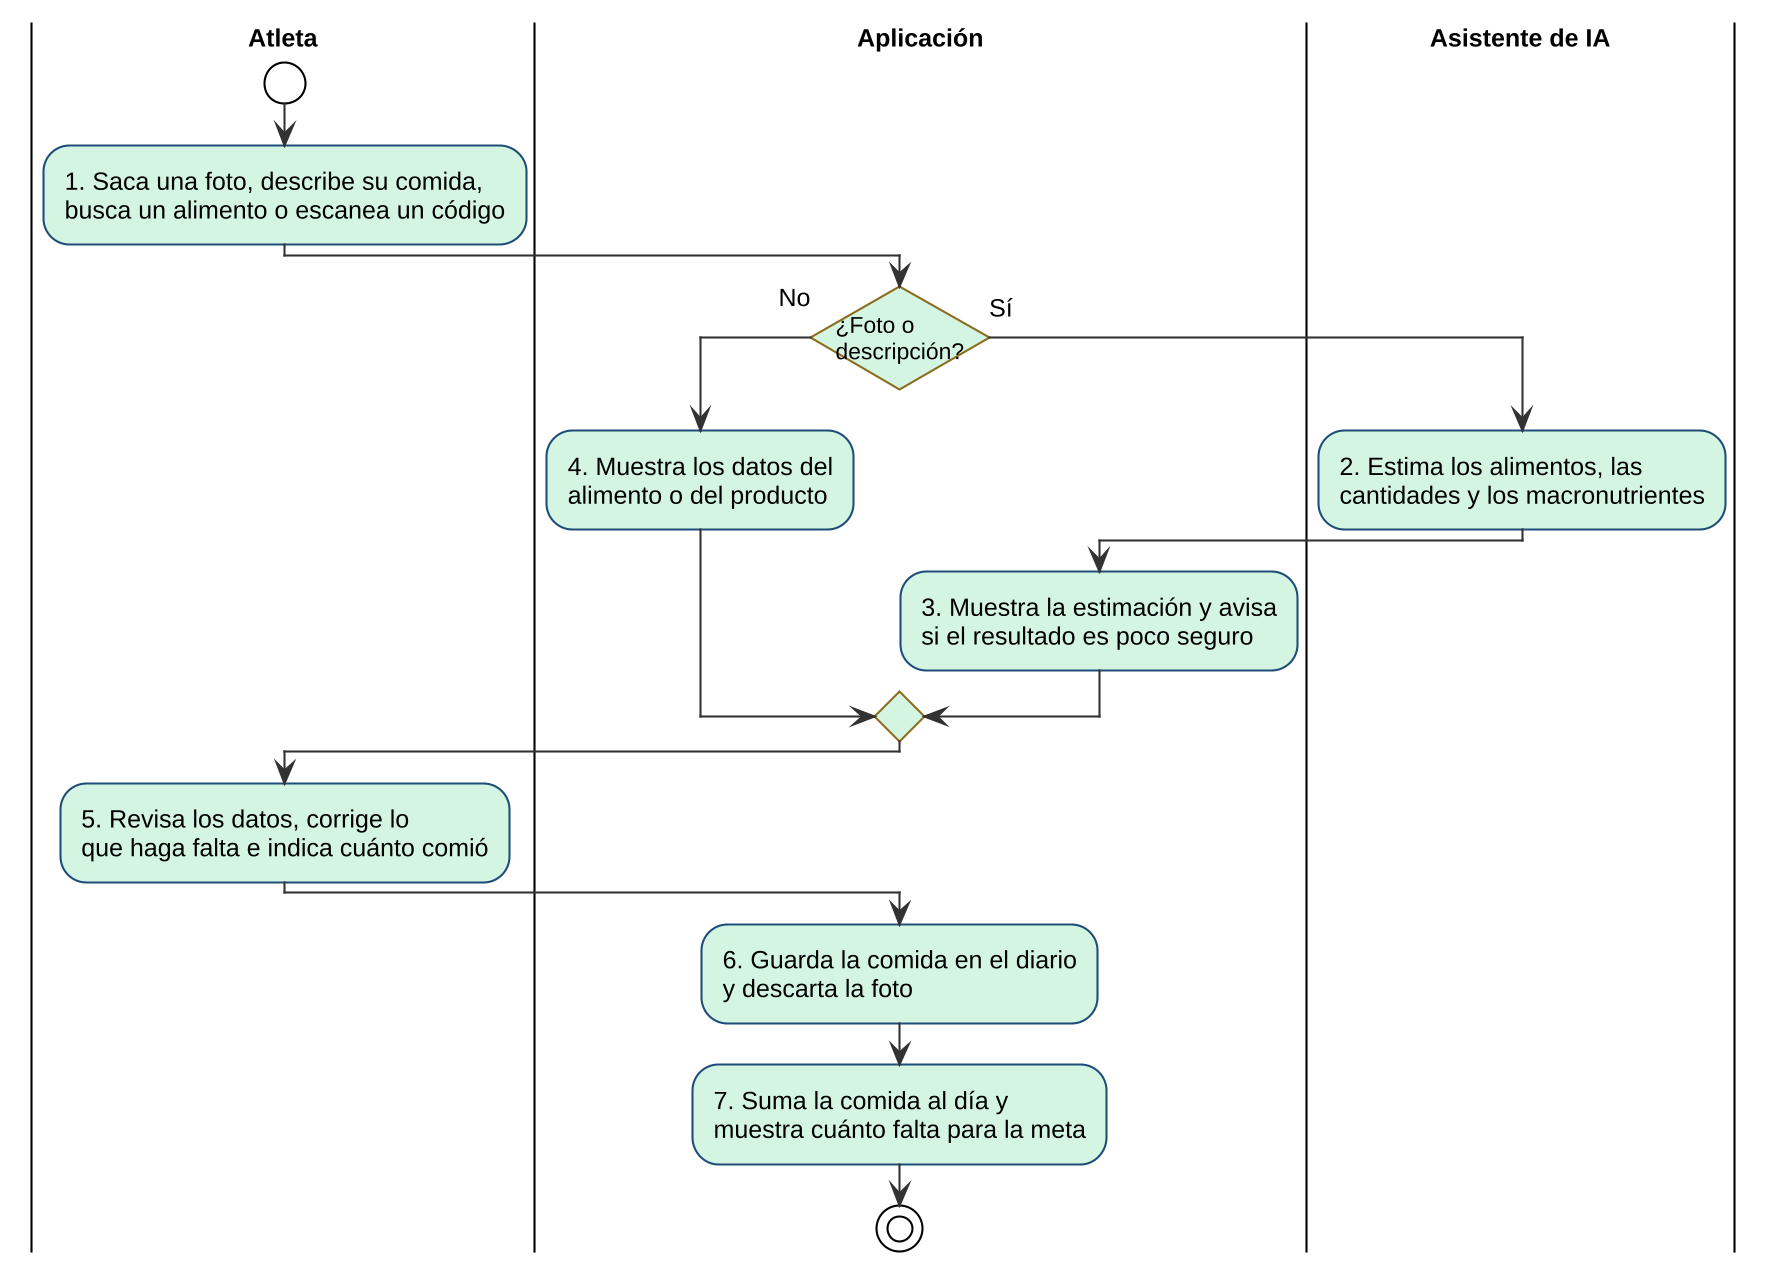
\includegraphics[width=0.9\textwidth]{figuras/procesos/bpmn_proceso2.png}
    \caption{Proceso 2: Registro de comidas y metas de alimentación.}
    \label{fig:bpmn_nutricion}
\end{figure}

\textbf{Tareas del proceso}

\begin{enumerate}
    \item \textbf{Elige cómo registrar:} El atleta saca una foto a su plato, describe su comida con sus palabras, busca un alimento en la lista o escanea el código de barras de un producto.
    \item \textbf{Estima la comida:} Si usó una foto o una descripción, el asistente de IA estima los alimentos, las cantidades, las calorías y los macronutrientes.
    \item \textbf{Muestra la estimación:} La aplicación muestra el resultado y avisa cuando es poco seguro, para que el atleta lo revise con más cuidado.
    \item \textbf{Muestra los datos del alimento:} Si buscó un alimento o escaneó un código, la aplicación muestra sus calorías y macronutrientes.
    \item \textbf{Revisa y corrige:} En todos los casos el atleta revisa los datos, corrige lo que haga falta e indica cuánto comió. Nada se guarda sin que lo confirme.
    \item \textbf{Guarda la comida:} La comida queda en el diario del día. La foto se descarta después del análisis, salvo que el atleta la quiera publicar.
    \item \textbf{Muestra el avance:} La aplicación suma la comida al día y muestra cuánto falta para las metas calculadas en el Proceso 1. También puede sugerir en qué momento conviene comer, por ejemplo proteína después de una sesión de fuerza.
\end{enumerate}

La búsqueda en la lista y el código de barras son parte del plan gratuito. La foto, la descripción y las metas según el entrenamiento son parte del plan premium.
\newpage
\subsubsection{Proceso 3: Publicación y Uso de Contenido de la Comunidad}
Este proceso muestra cómo una sesión, una ruta o una comida que publica un atleta llega a otro, que puede agregarla a sus propios módulos o reportarla. Los participantes son el atleta que publica, el atleta que ve la publicación, la aplicación y el administrador. Responde a los requerimientos R08, R11 y R12.

\begin{figure}[h!]
    \centering
    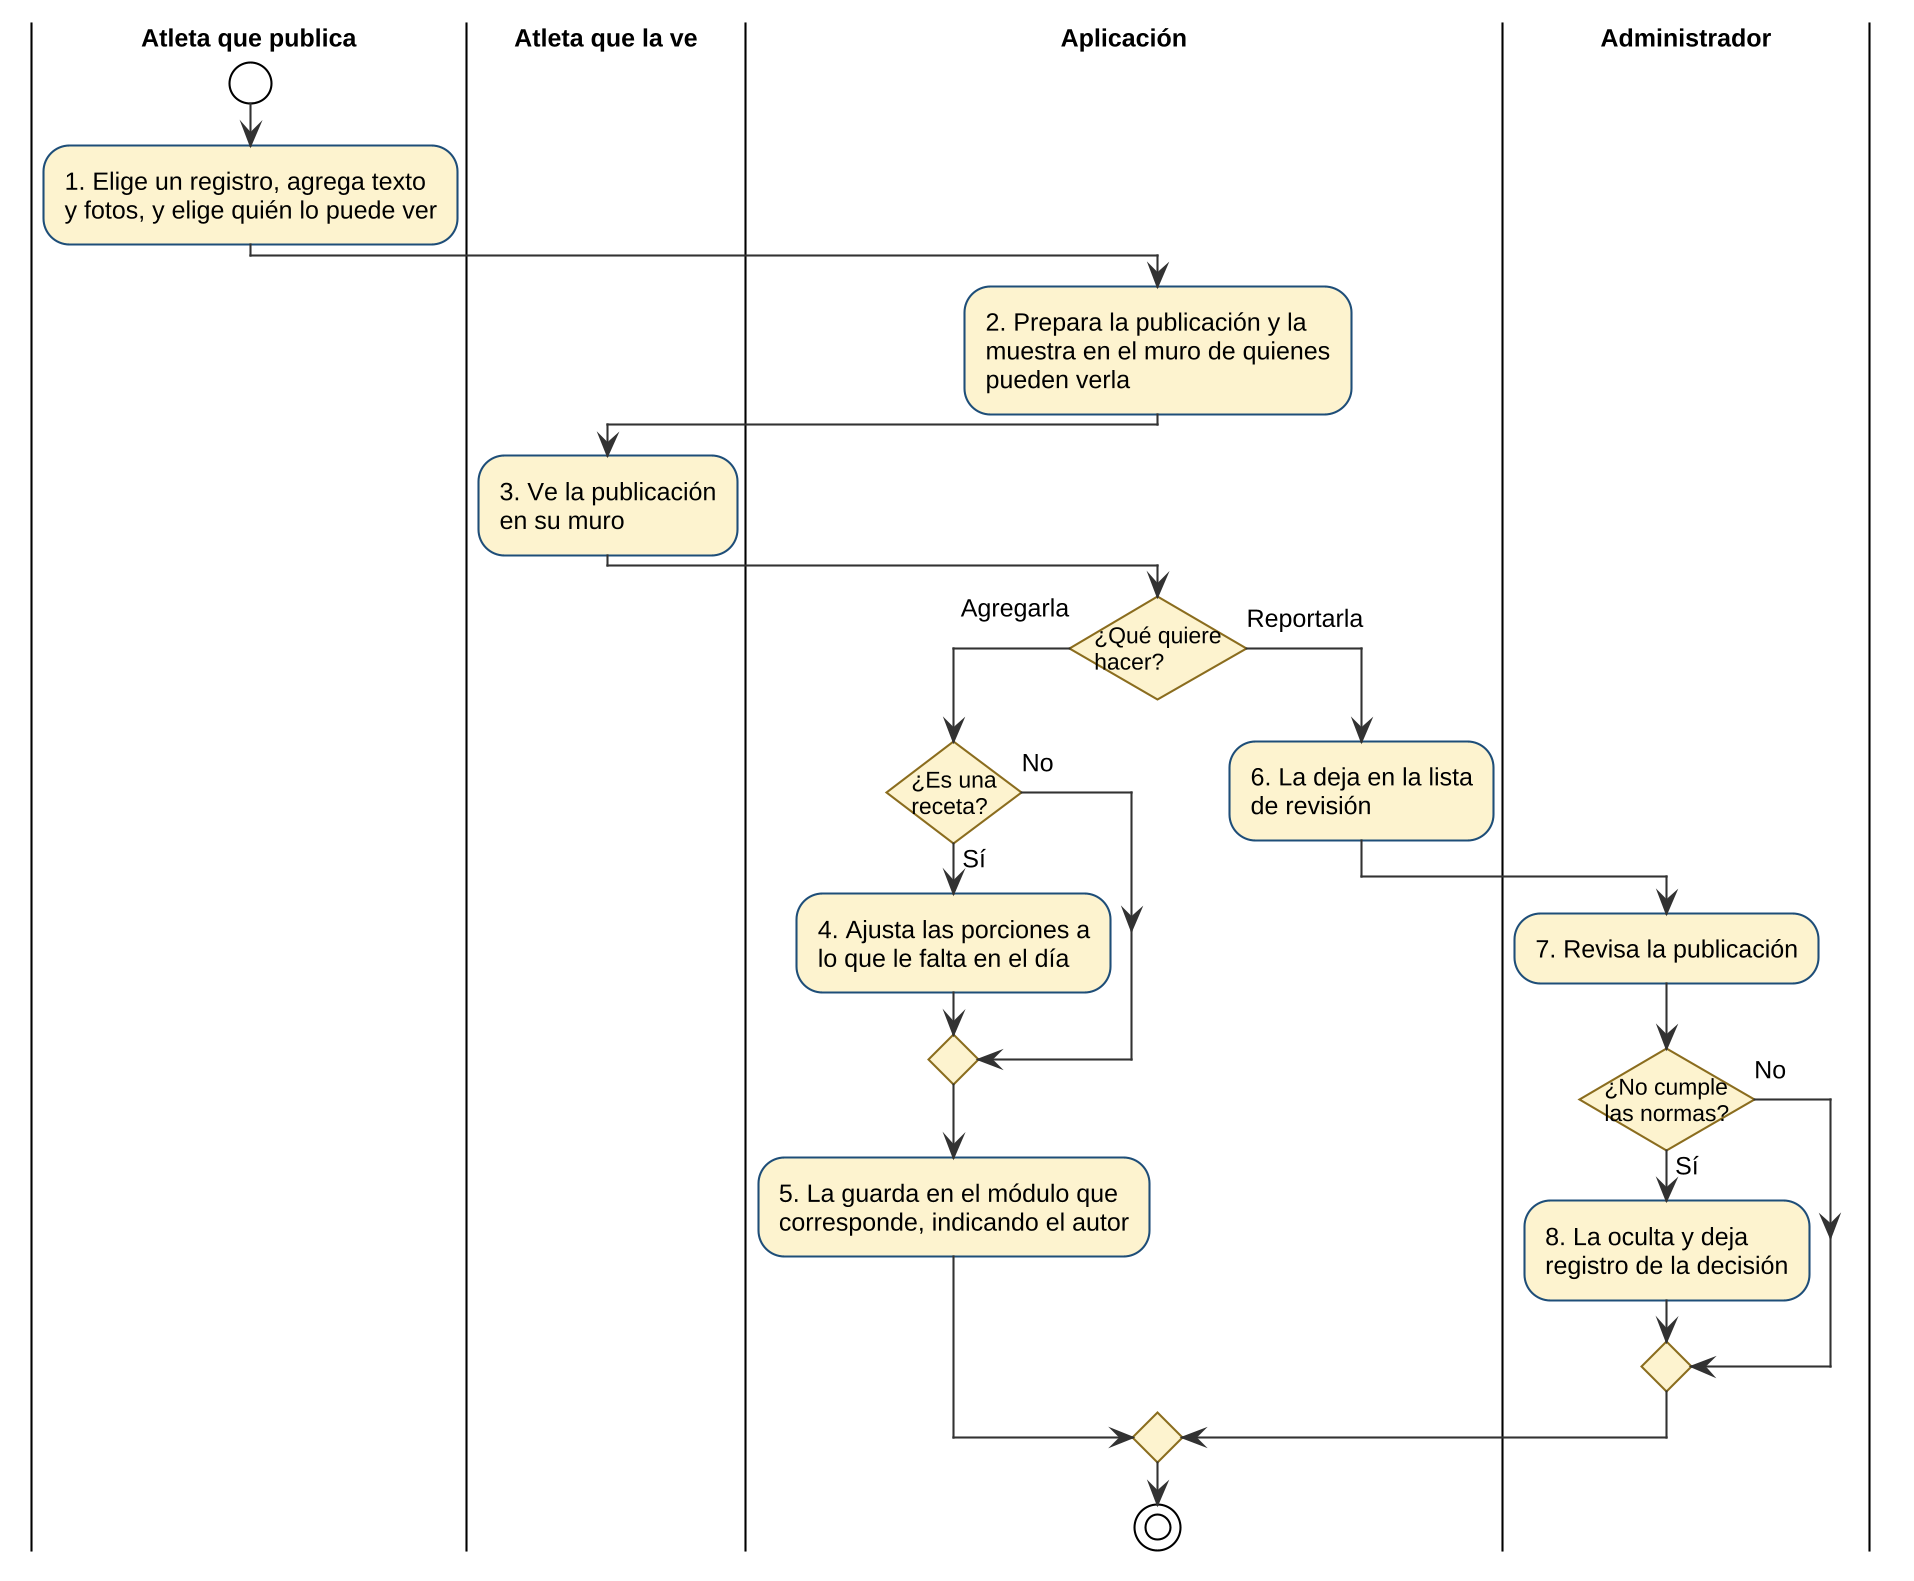
\includegraphics[width=0.85\textwidth]{figuras/procesos/bpmn_proceso3.png}
    \caption{Proceso 3: Publicación y uso de contenido de la comunidad.}
    \label{fig:bpmn_recetas}
\end{figure}
\newpage
\textbf{Tareas del proceso}

\begin{enumerate}
    \item \textbf{Publica un registro:} El atleta elige una sesión, una ruta o una comida que ya registró, le agrega un texto y hasta 4 fotos, y elige quién la puede ver (todos, sus seguidores o solo él).
    \item \textbf{Prepara y muestra la publicación:} La aplicación comprime las fotos, les borra los datos de ubicación y, si es una ruta, oculta el inicio y el final del recorrido. Luego la publicación aparece en el muro de quienes pueden verla.
    \item \textbf{Ve la publicación:} Otro atleta la encuentra en su muro. Si le interesa, puede agregarla a sus módulos o reportarla.
    \item \textbf{Ajusta las porciones:} Si agrega una receta, la aplicación ajusta la cantidad de cada ingrediente según lo que le falta comer ese día, manteniendo las proporciones de la receta original.
    \item \textbf{Guarda en el módulo que corresponde:} Una sesión de fuerza queda como rutina, una ruta queda en cardio y una receta queda en nutrición, siempre indicando quién la creó. Agregar una receta no la registra como comida. Eso ocurre cuando el atleta se la come y la anota en su diario (Proceso 2).
    \item \textbf{Deja la publicación en revisión:} Si el atleta la reporta, indica el motivo y la publicación pasa a la lista de revisión del administrador.
    \item \textbf{Revisa la publicación:} El administrador evalúa si cumple las normas de la comunidad o si puede ser peligrosa para la salud.
    \item \textbf{Oculta la publicación:} Si no cumple las normas, el administrador la oculta y queda registro de quién tomó la decisión y por qué.
\end{enumerate}
\newpage
\subsubsection{Proceso 4: Registro de Fuerza}
Este proceso muestra las dos formas de registrar una sesión de fuerza, ya sea con el formulario o con las propias palabras del atleta, para que anotar una sesión tome poco tiempo. Los participantes son el atleta, la aplicación y el asistente de inteligencia artificial. Responde al requerimiento R01.

\begin{figure}[h!]
    \centering
    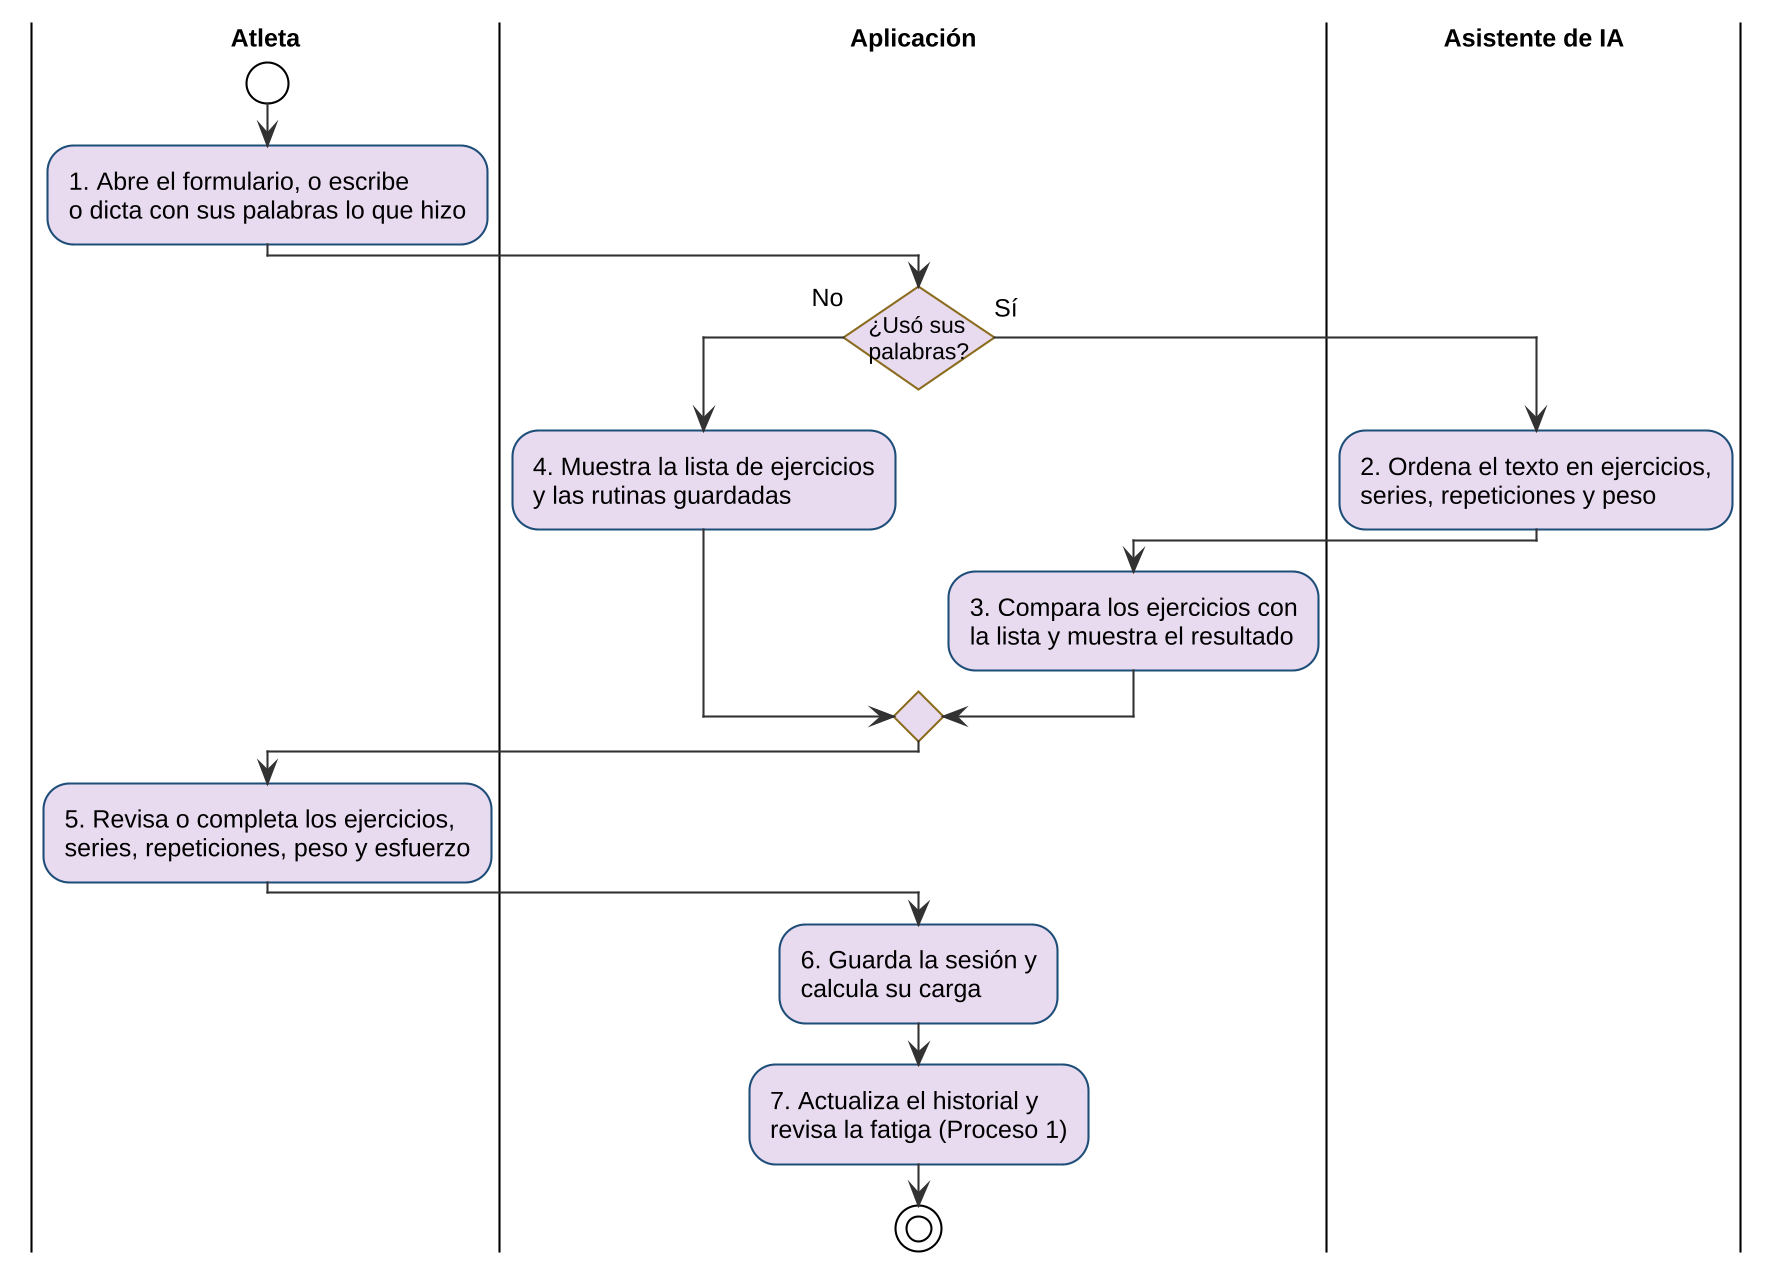
\includegraphics[width=0.9\textwidth]{figuras/procesos/bpmn_proceso4.png}
    \caption{Proceso 4: Registro de fuerza.}
    \label{fig:bpmn_nlp}
\end{figure}

\textbf{Tareas del proceso}

\begin{enumerate}
    \item \textbf{Elige cómo registrar:} El atleta abre el formulario, o escribe o dicta lo que hizo, por ejemplo ``hice 4 series de 8 sentadillas con 100 kilos''.
    \item \textbf{Ordena el texto:} Si usó sus palabras, el asistente de IA separa el texto en ejercicios, series, repeticiones y peso.
    \item \textbf{Compara con la lista:} La aplicación busca cada ejercicio en su lista y muestra el resultado.
    \item \textbf{Muestra la lista y las rutinas:} Si usó el formulario, la aplicación muestra la lista de ejercicios y las rutinas que el atleta tiene guardadas.
    \item \textbf{Revisa o completa:} El atleta confirma o completa los ejercicios, las series, las repeticiones, el peso y qué tan duro lo sintió (RPE). Nada se guarda sin que lo confirme.
    \item \textbf{Guarda la sesión:} La aplicación guarda la sesión y calcula su carga.
    \item \textbf{Actualiza el historial y revisa la fatiga:} La sesión aparece en el historial. Con esta carga se repite el cruce de datos desde la tarea 5 del Proceso 1, de modo que una sesión de fuerza también puede generar una alerta antes de una sesión exigente de cardio.
\end{enumerate}

El formulario es parte del plan gratuito. El registro con las propias palabras y el cruce de datos son parte del plan premium.
\newpage
\subsubsection{Proceso 5: Perfil del Usuario y Plan Sugerido}
Este proceso muestra cómo la aplicación conoce a un usuario nuevo, le sugiere un plan de entrenamiento y lo va ajustando cada semana con lo que registra. Es el proceso que da una guía a quien recién empieza. Los participantes son el atleta y la aplicación. Responde al requerimiento R13.

\begin{figure}[h!]
    \centering
    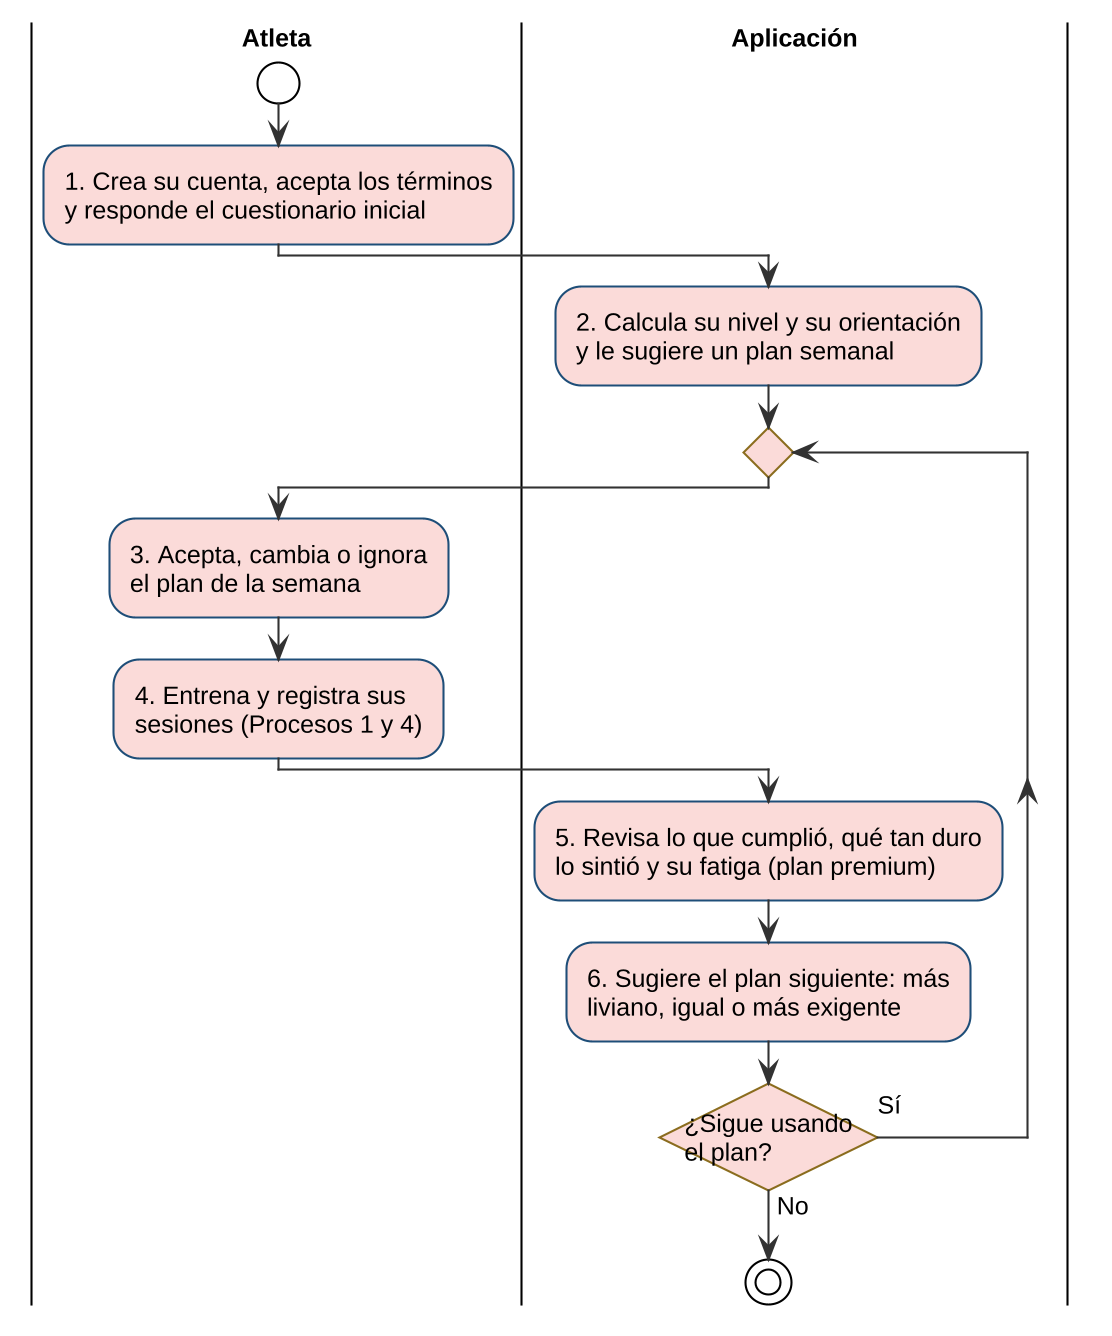
\includegraphics[width=0.62\textwidth]{figuras/procesos/bpmn_proceso5.png}
    \caption{Proceso 5: Perfil del usuario y plan sugerido.}
    \label{fig:bpmn_plan}
\end{figure}

\textbf{Tareas del proceso}

\begin{enumerate}
    \item \textbf{Crea su cuenta y responde el cuestionario:} El atleta acepta los términos de uso y el aviso legal, y responde preguntas sobre su experiencia, sus objetivos, los días que puede entrenar, su equipamiento, las disciplinas que practica, su edad, su sexo, su estatura y su peso.
    \item \textbf{Calcula su nivel y sugiere un plan:} La aplicación lo clasifica según su nivel (principiante, intermedio o avanzado) y su orientación (más fuerza, más resistencia o equilibrada), y le sugiere un plan semanal a partir de una plantilla para ese perfil.
    \item \textbf{Acepta, cambia o ignora el plan:} El plan es una sugerencia, y la decisión siempre es del atleta.
    \item \textbf{Entrena y registra:} Durante la semana registra sus sesiones, como se explica en los Procesos 1 y 4.
    \item \textbf{Revisa la semana:} La aplicación compara las sesiones cumplidas con las sugeridas y revisa qué tan duro las sintió el atleta. En el plan premium también considera su fatiga cruzada.
    \item \textbf{Sugiere el plan siguiente:} Con reglas simples, la aplicación propone un plan más liviano, igual o más exigente, y explica por qué cambió. El ciclo se repite cada semana mientras el atleta siga usando el plan.
\end{enumerate}
\newpage
\subsection{Modelo de Requerimientos}
El Modelo de Requerimientos reúne lo que el sistema debe hacer de cara al usuario (requerimientos funcionales) y la forma técnica en que se va a lograr (requerimientos no funcionales). A continuación se presenta el diagrama de trazabilidad, que relaciona los procesos de negocio de la sección anterior (cardio y fatiga, comidas y metas, comunidad, registro de fuerza y plan sugerido) con los requerimientos funcionales que los hacen posibles. Los requerimientos que no pertenecen a un proceso en particular se agrupan como funciones transversales de la plataforma.

\begin{figure}[h!]
    \centering
    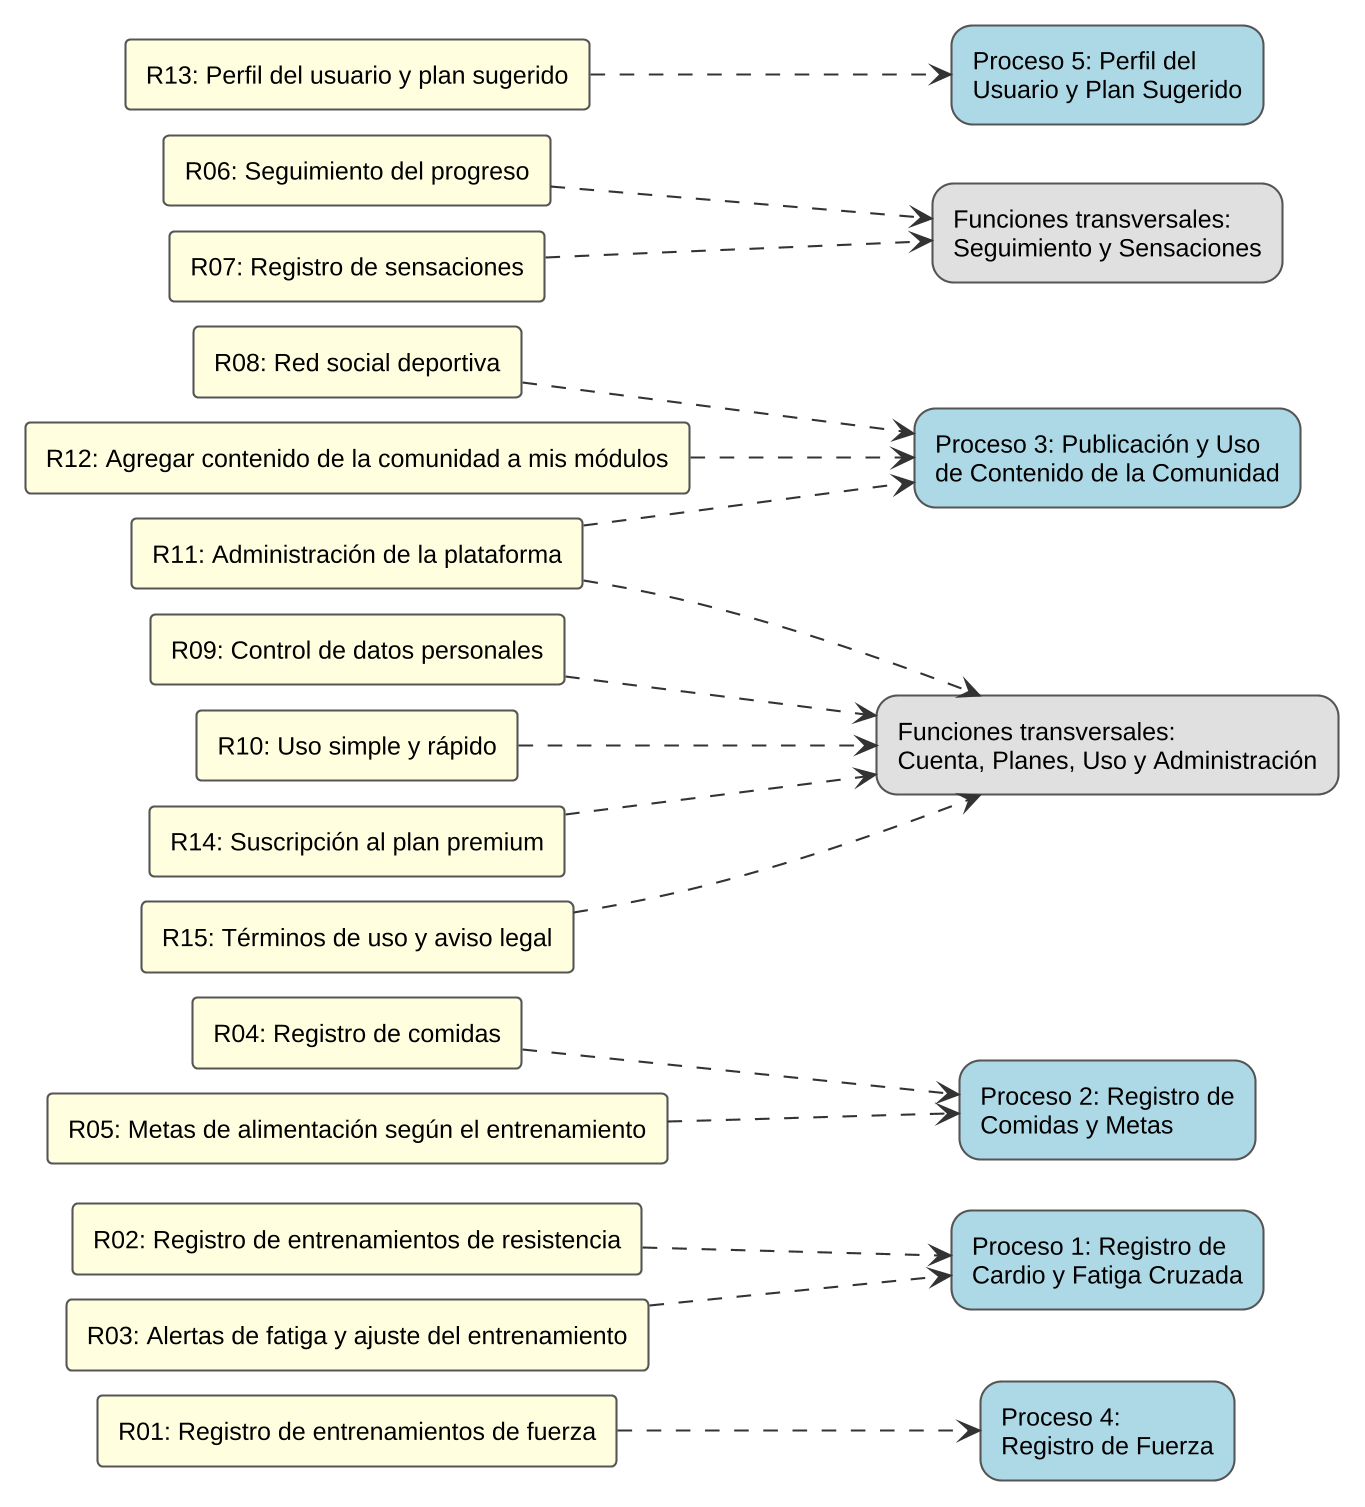
\includegraphics[width=0.8\textwidth]{figuras/requerimientos/diagrama_requerimientos.png}
    \caption{Diagrama de trazabilidad: relación entre requerimientos y procesos de negocio.}
    \label{fig:diagrama_requerimientos}
\end{figure}
\newpage
\subsubsection{Requerimientos Funcionales}
Los requerimientos funcionales describen lo que la aplicación permite hacer al usuario y lo que le entrega a cambio. Se presentan en quince requerimientos, escritos desde el punto de vista de quien usa la aplicación y no de los procesos internos del sistema. Catorce corresponden al deportista y uno al administrador de la plataforma.

\begin{table}[h!]
    \centering
    \renewcommand{\arraystretch}{1.3}
    \begin{tabular}{|p{3.5cm}|p{11.5cm}|}
        \hline
        \rowcolor[HTML]{EFEFEF} 
        \textbf{Identificador} & \textbf{R01} \\ \hline
        \textbf{Nombre} & Registro de entrenamientos de fuerza \\ \hline
        \textbf{Descripción} & La aplicación debe permitir al usuario registrar sus sesiones de fuerza. Puede elegir los ejercicios desde un catálogo e ingresar las series, repeticiones, peso y esfuerzo percibido (RPE), o describir la sesión con sus propias palabras, escribiéndola o dictándola. \\ \hline
        \textbf{Prioridad} & Alta \\ \hline
    \end{tabular}
\end{table}

\begin{table}[h!]
    \centering
    \renewcommand{\arraystretch}{1.3}
    \begin{tabular}{|p{3.5cm}|p{11.5cm}|}
        \hline
        \rowcolor[HTML]{EFEFEF} 
        \textbf{Identificador} & \textbf{R02} \\ \hline
        \textbf{Nombre} & Registro de entrenamientos de resistencia \\ \hline
        \textbf{Descripción} & La aplicación debe permitir al usuario registrar sus sesiones de ciclismo, running y trekking. Los datos pueden provenir del GPS del teléfono, de su reloj o ciclocomputador, o de un archivo exportado desde estos dispositivos. Si no cuenta con datos de un dispositivo, puede registrar la sesión indicando cómo sintió el esfuerzo. \\ \hline
        \textbf{Prioridad} & Alta \\ \hline
    \end{tabular}
\end{table}

\begin{table}[h!]
    \centering
    \renewcommand{\arraystretch}{1.3}
    \begin{tabular}{|p{3.5cm}|p{11.5cm}|}
        \hline
        \rowcolor[HTML]{EFEFEF} 
        \textbf{Identificador} & \textbf{R03} \\ \hline
        \textbf{Nombre} & Alertas de fatiga y ajuste del entrenamiento \\ \hline
        \textbf{Descripción} & La aplicación debe cruzar las métricas de esfuerzo de las sesiones de fuerza y de resistencia del usuario. Con esa información, debe avisarle cuando exista un posible estado de fatiga, por ejemplo si tiene una sesión de fuerza máxima programada después de un entrenamiento de resistencia muy exigente, y sugerirle cómo ajustar sus próximos entrenamientos. También debe avisarle cuando deje poco tiempo de recuperación entre sesiones de distinto tipo, y considerar en la alerta si viene comiendo bastante menos de lo que gasta. \\ \hline
        \textbf{Prioridad} & Crítica \\ \hline
    \end{tabular}
\end{table}
\newpage
\begin{table}[h!]
    \centering
    \renewcommand{\arraystretch}{1.3}
    \begin{tabular}{|p{3.5cm}|p{11.5cm}|}
        \hline
        \rowcolor[HTML]{EFEFEF} 
        \textbf{Identificador} & \textbf{R04} \\ \hline
        \textbf{Nombre} & Registro de comidas \\ \hline
        \textbf{Descripción} & La aplicación debe permitir al usuario registrar lo que come de cuatro formas: buscando alimentos en un listado, describiéndolos con sus propias palabras, sacando una foto al plato o leyendo el código de barras de un producto comercial. En todos los casos, debe mostrar las calorías y los macronutrientes para que el usuario pueda revisarlos y corregirlos. \\ \hline
        \textbf{Prioridad} & Alta \\ \hline
    \end{tabular}
\end{table}

\begin{table}[h!]
    \centering
    \renewcommand{\arraystretch}{1.3}
    \begin{tabular}{|p{3.5cm}|p{11.5cm}|}
        \hline
        \rowcolor[HTML]{EFEFEF} 
        \textbf{Identificador} & \textbf{R05} \\ \hline
        \textbf{Nombre} & Metas de alimentación según el entrenamiento \\ \hline
        \textbf{Descripción} & La aplicación debe mostrar al usuario metas diarias de calorías y macronutrientes que cambien según el entrenamiento realizado o planificado, por ejemplo con más carbohidratos después de una ruta larga en bicicleta. También debe sugerirle en qué momento conviene comer respecto al entrenamiento. Estas metas son una sugerencia, y el usuario decide cómo seguirlas. La aplicación no entrega dietas ni planes de alimentación prescritos. \\ \hline
        \textbf{Prioridad} & Media \\ \hline
    \end{tabular}
\end{table}

\begin{table}[h!]
    \centering
    \renewcommand{\arraystretch}{1.3}
    \begin{tabular}{|p{3.5cm}|p{11.5cm}|}
        \hline
        \rowcolor[HTML]{EFEFEF} 
        \textbf{Identificador} & \textbf{R06} \\ \hline
        \textbf{Nombre} & Seguimiento del progreso \\ \hline
        \textbf{Descripción} & La aplicación debe mostrar al usuario, en una línea de tiempo diaria y mensual, sus entrenamientos, su alimentación y su carga acumulada, para que pueda revisar su progreso en un solo lugar. \\ \hline
        \textbf{Prioridad} & Alta \\ \hline
    \end{tabular}
\end{table}

\begin{table}[h!]
    \centering
    \renewcommand{\arraystretch}{1.3}
    \begin{tabular}{|p{3.5cm}|p{11.5cm}|}
        \hline
        \rowcolor[HTML]{EFEFEF} 
        \textbf{Identificador} & \textbf{R07} \\ \hline
        \textbf{Nombre} & Registro de sensaciones \\ \hline
        \textbf{Descripción} & La aplicación debe permitir al usuario anotar, en texto libre, cómo se sintió física y digestivamente, y asociar esa anotación a un entrenamiento o a una comida. \\ \hline
        \textbf{Prioridad} & Baja \\ \hline
    \end{tabular}
\end{table}
\newpage
\begin{table}[h!]
    \centering
    \renewcommand{\arraystretch}{1.3}
    \begin{tabular}{|p{3.5cm}|p{11.5cm}|}
        \hline
        \rowcolor[HTML]{EFEFEF} 
        \textbf{Identificador} & \textbf{R08} \\ \hline
        \textbf{Nombre} & Red social deportiva \\ \hline
        \textbf{Descripción} & La aplicación debe permitir al usuario seguir a otras personas, ver un muro con sus publicaciones y publicar en su perfil sus sesiones de fuerza, sus rutas y sus comidas o recetas, eligiendo si cada publicación es pública, solo para sus seguidores o privada. Cada publicación puede incluir fotos. Esta función está disponible para usuarios premium. \\ \hline
        \textbf{Prioridad} & Alta \\ \hline
    \end{tabular}
\end{table}

\begin{table}[h!]
    \centering
    \renewcommand{\arraystretch}{1.3}
    \begin{tabular}{|p{3.5cm}|p{11.5cm}|}
        \hline
        \rowcolor[HTML]{EFEFEF} 
        \textbf{Identificador} & \textbf{R09} \\ \hline
        \textbf{Nombre} & Control de datos personales \\ \hline
        \textbf{Descripción} & Antes de acceder a sus datos de salud, la aplicación debe pedir al usuario su autorización de forma clara. Además, el usuario debe poder consultar, corregir y eliminar sus datos, y eliminar su cuenta por completo cuando lo necesite. \\ \hline
        \textbf{Prioridad} & Alta \\ \hline
    \end{tabular}
\end{table}

\begin{table}[h!]
    \centering
    \renewcommand{\arraystretch}{1.3}
    \begin{tabular}{|p{3.5cm}|p{11.5cm}|}
        \hline
        \rowcolor[HTML]{EFEFEF} 
        \textbf{Identificador} & \textbf{R10} \\ \hline
        \textbf{Nombre} & Uso simple y rápido \\ \hline
        \textbf{Descripción} & El usuario debe poder registrar una sesión o una comida en pocos pasos. La respuesta de la aplicación, incluida la estimación de una foto de comida, debe ser rápida, y la experiencia debe ser la misma en Android y en iOS. \\ \hline
        \textbf{Prioridad} & Media \\ \hline
    \end{tabular}
\end{table}
\begin{table}[h!]
    \centering
    \renewcommand{\arraystretch}{1.3}
    \begin{tabular}{|p{3.5cm}|p{11.5cm}|}
        \hline
        \rowcolor[HTML]{EFEFEF} 
        \textbf{Identificador} & \textbf{R11} \\ \hline
        \textbf{Nombre} & Administración de la plataforma \\ \hline
        \textbf{Descripción} & La aplicación debe contar con un panel para el administrador, donde pueda mantener actualizado el catálogo de ejercicios (crear, editar y eliminar ejercicios) y revisar lo que publican los usuarios, eliminando las publicaciones, fotos o recetas que incumplan las normas de la comunidad o representen un riesgo para la salud. \\ \hline
        \textbf{Prioridad} & Media \\ \hline
    \end{tabular}
\end{table}
\newpage
\begin{table}[h!]
    \centering
    \renewcommand{\arraystretch}{1.3}
    \begin{tabular}{|p{3.5cm}|p{11.5cm}|}
        \hline
        \rowcolor[HTML]{EFEFEF} 
        \textbf{Identificador} & \textbf{R12} \\ \hline
        \textbf{Nombre} & Agregar contenido de la comunidad a mis módulos \\ \hline
        \textbf{Descripción} & La aplicación debe permitir al usuario agregar con un botón cualquier publicación de la comunidad a su módulo correspondiente, sin copiarla a mano. Una sesión de fuerza se guarda como una rutina propia, una ruta pasa a su módulo de cardio y una receta pasa a su módulo de nutrición, con las porciones ajustadas a sus necesidades del día. \\ \hline
        \textbf{Prioridad} & Alta \\ \hline
    \end{tabular}
\end{table}

\begin{table}[h!]
    \centering
    \renewcommand{\arraystretch}{1.3}
    \begin{tabular}{|p{3.5cm}|p{11.5cm}|}
        \hline
        \rowcolor[HTML]{EFEFEF} 
        \textbf{Identificador} & \textbf{R13} \\ \hline
        \textbf{Nombre} & Perfil del usuario y plan sugerido \\ \hline
        \textbf{Descripción} & Al registrarse, la aplicación debe preguntar al usuario por su experiencia, sus objetivos, los días que tiene disponibles, su equipamiento y las disciplinas que practica, además de su edad, su sexo, su estatura y su peso, que se necesitan para estimar su gasto de energía. Con esa información debe sugerirle un plan semanal de entrenamiento adaptado a su nivel, que se ajuste con lo que registra. El plan es una sugerencia, y el usuario puede modificarlo o ignorarlo. \\ \hline
        \textbf{Prioridad} & Alta \\ \hline
    \end{tabular}
\end{table}
\newpage
\begin{table}[h!]
    \centering
    \renewcommand{\arraystretch}{1.3}
    \begin{tabular}{|p{3.5cm}|p{11.5cm}|}
        \hline
        \rowcolor[HTML]{EFEFEF}
        \textbf{Identificador} & \textbf{R14} \\ \hline
        \textbf{Nombre} & Suscripción al plan premium \\ \hline
        \textbf{Descripción} & La aplicación debe permitir al usuario contratar el plan premium y cancelarlo cuando quiera. Antes de contratar, debe mostrarle el precio final con impuestos incluidos y cada cuánto se cobra. Para cancelar, la aplicación debe llevarlo a la pantalla de suscripciones de su tienda, donde confirma la cancelación sin necesidad de hablar con una persona. Al terminar el periodo pagado, el usuario vuelve al plan gratuito y conserva sus datos. \\ \hline
        \textbf{Prioridad} & Alta \\ \hline
    \end{tabular}
\end{table}

\begin{table}[h!]
    \centering
    \renewcommand{\arraystretch}{1.3}
    \begin{tabular}{|p{3.5cm}|p{11.5cm}|}
        \hline
        \rowcolor[HTML]{EFEFEF}
        \textbf{Identificador} & \textbf{R15} \\ \hline
        \textbf{Nombre} & Términos de uso y aviso legal \\ \hline
        \textbf{Descripción} & Al crear su cuenta, la aplicación debe mostrar al usuario los términos de uso y el aviso legal, y pedirle que los acepte antes de seguir. Los términos deben explicar para qué se usan sus datos, que no se venden a terceros y que lo que publique se podrá mostrar a la comunidad y otros podrán agregarlo a sus módulos. El aviso debe dejar claro que la aplicación es un apoyo deportivo y que no reemplaza a un médico ni a un nutricionista. Al publicar una foto, el usuario debe declarar que es suya o que tiene permiso para publicarla. \\ \hline
        \textbf{Prioridad} & Alta \\ \hline
    \end{tabular}
\end{table}
\newpage

\subsubsection{Características de los Usuarios del Sistema}
El sistema contempla tres perfiles de usuario con niveles de acceso diferenciados, diseñados para cubrir desde el deportista principiante hasta la administración técnica de la plataforma.

\begin{table}[h!]
    \centering
    \renewcommand{\arraystretch}{1.3}
    \begin{tabular}{|p{3cm}|p{4cm}|p{7.5cm}|}
        \hline
        \rowcolor[HTML]{EFEFEF}
        \textbf{Perfil} & \textbf{Nivel de Acceso} & \textbf{Descripción} \\ \hline
        Atleta Básico (Free) & Funcionalidades esenciales & Deportista aficionado que utiliza la plataforma para el registro manual de entrenamientos de fuerza y de cardio y de sus comidas. No requiere dispositivos externos. Su experiencia técnica es baja a media y su objetivo principal es llevar un seguimiento ordenado de su actividad. Puede ser un deportista novato, que recibe un plan sugerido según su perfil. \\ \hline
        Atleta Híbrido (Premium) & Funcionalidades completas & Deportista que practica entrenamiento concurrente (fuerza + resistencia) y requiere el cruce de datos automatizado. Accede a la sincronización con wearables, el escáner nutricional por IA, el registro por NLP, el motor de fatiga cruzada y la red social deportiva. Posee experiencia media a alta con tecnología deportiva. \\ \hline
        Administrador & Panel de gestión interno & Perfil técnico responsable de la curación de la base de datos maestra de ejercicios, la moderación del contenido generado por la comunidad (recetas y publicaciones), y el monitoreo de métricas operativas del sistema (logs, rendimiento de la API, uso de cuotas de IA). \\ \hline
    \end{tabular}
    \caption{Perfiles de usuario del sistema.}
    \label{tab:perfiles_usuario}
\end{table}

La Tabla \ref{tab:funciones_plan} resume qué incluye cada plan.

\begin{table}[h!]
    \centering
    \renewcommand{\arraystretch}{1.3}
    \begin{tabular}{|>{\raggedright\arraybackslash}p{7.5cm}|>{\raggedright\arraybackslash}p{3.5cm}|>{\raggedright\arraybackslash}p{3.5cm}|}
        \hline
        \rowcolor[HTML]{EFEFEF}
        \textbf{Función} & \textbf{Plan gratuito} & \textbf{Plan premium} \\ \hline
        Cuestionario y plan semanal sugerido & Sí, se ajusta con lo cumplido y el RPE & Sí, y además con la fatiga \\ \hline
        Registro manual de fuerza, cardio (GPS o a mano) y comidas, con código de barras & Sí & Sí \\ \hline
        Progreso, sensaciones y control de datos personales & Sí & Sí \\ \hline
        Lectura desde el reloj y archivos \texttt{.fit} & No & Sí \\ \hline
        Registro con inteligencia artificial & No & Sí \\ \hline
        Cruce de datos, alertas de fatiga y metas de alimentación & No & Sí \\ \hline
        Red social deportiva & No & Sí \\ \hline
    \end{tabular}
    \caption{Funciones de cada plan.}
    \label{tab:funciones_plan}
\end{table}
\newpage
\subsubsection{Propósito del Sistema}
El propósito del sistema es centralizar la captura, el almacenamiento y el análisis cruzado de datos provenientes de tres dominios históricamente fragmentados: el entrenamiento de fuerza, la resistencia cardiovascular y la nutrición deportiva. A través de la integración de telemetría de wearables, inteligencia artificial (visión computacional y procesamiento de lenguaje natural) y un motor algorítmico de fatiga concurrente, la plataforma busca:
\begin{enumerate}
    \item Facilitar el registro de sesiones deportivas y comidas, reduciendo la fricción operativa que genera el uso simultáneo de múltiples aplicaciones aisladas.
    \item Cuantificar objetivamente la fatiga cruzada entre disciplinas, permitiendo al atleta híbrido prevenir el sobreentrenamiento y el efecto de interferencia sin depender de estimaciones subjetivas.
    \item Adaptar dinámicamente los objetivos nutricionales diarios en función del desgaste fisiológico real, abandonando los modelos estáticos de calorías que no distinguen entre un día de descanso y un fondo largo en bicicleta.
    \item Entregar información personalizada, con un plan semanal sugerido según el perfil de cada usuario, incluso si no tiene experiencia previa.
    \item Fomentar la adherencia a largo plazo mediante una red social deportiva, donde el contenido que publican otros usuarios se puede agregar directamente a los propios módulos.
\end{enumerate}
\newpage
\subsubsection{Restricciones Generales}
Las siguientes restricciones condicionan el diseño, desarrollo y operación de la solución tecnológica:

\begin{itemize}
    \item \textbf{Dependencia de conectividad a Internet:} Los servicios de inteligencia artificial (visión y NLP) operan en la nube. El procesamiento de imágenes de alimentos y la interpretación de texto en lenguaje natural requieren una conexión activa a Internet. El registro manual de datos podrá funcionar con conectividad limitada mediante un sistema de cola local que sincronice al recuperar la conexión.
    \item \textbf{Restricción sanitaria y legal:} De acuerdo con el Código Sanitario (DFL N° 725) y la Ley N° 20.584, el sistema no emitirá diagnósticos médicos, prescripciones clínicas ni planes dietoterapéuticos. Todas las recomendaciones algorítmicas se presentarán como sugerencias de optimización deportiva, acompañadas de un disclaimer legal permanente.
    \item \textbf{Protección de datos sensibles:} El tratamiento de biomarcadores (frecuencia cardíaca, peso corporal, ubicación GPS) debe cumplir íntegramente con la Ley N° 19.628 sobre Protección de la Vida Privada, implementando consentimiento explícito, derechos ARCO y cifrado obligatorio.
    \item \textbf{Dependencia de hardware de terceros:} La plataforma no desarrolla dispositivos propios. La captura de telemetría cardiovascular depende de la disponibilidad y compatibilidad de wearables comerciales (Garmin, Polar, Apple Watch) y de los SDKs de Health Connect y Apple HealthKit.
    \item \textbf{Disciplinas deportivas acotadas:} El módulo de resistencia se limita exclusivamente a ciclismo, running y trekking. No se contempla soporte para natación, remo u otras disciplinas de resistencia.
    \item \textbf{Cuotas de API externas:} El consumo de la API de Gemini está sujeto a límites de uso (rate limits) y costos por token. El diseño del backend debe implementar mecanismos de caché y control de gasto para evitar sobrecostos operativos.
\end{itemize}
\newpage
\subsubsection{Requisitos Específicos del Producto}
Los requisitos específicos detallan las capacidades particulares que cada módulo del producto debe ofrecer para satisfacer los requerimientos funcionales previamente definidos.

\begin{itemize}
    \item \textbf{Módulo de Fuerza:}
    \begin{itemize}
        \item El sistema debe mantener una base de datos maestra con al menos 200 ejercicios categorizados por grupo muscular, patrón de movimiento y equipamiento requerido.
        \item El usuario debe poder crear ejercicios personalizados que se almacenen en su perfil individual.
        \item Cada serie registrada debe contener como mínimo: ejercicio, peso (kg), repeticiones y, opcionalmente, RPE (escala 1--10).
        \item El registro por NLP debe soportar la entrada de múltiples ejercicios en un solo bloque de texto.
    \end{itemize}
    \item \textbf{Módulo de Resistencia (Cardio):}
    \begin{itemize}
        \item El sistema debe sincronizar automáticamente las sesiones de ciclismo, running y trekking registradas en Health Connect o Apple HealthKit.
        \item El parser de archivos \texttt{.fit} debe extraer, como mínimo: duración, distancia, frecuencia cardíaca promedio y máxima, potencia promedio (si aplica), cadencia y Training Stress Score (TSS).
        \item La telemetría segundo a segundo debe almacenarse en una colección de series temporales (\texttt{telemetry}) asociada a la sesión.
    \end{itemize}
    \item \textbf{Módulo de Nutrición:}
    \begin{itemize}
        \item El escáner de visión artificial debe retornar una estimación de calorías totales, proteínas (g), carbohidratos (g) y grasas (g) junto con un índice de confianza (0--100\%).
        \item Si el índice de confianza es inferior al 70\%, el sistema debe solicitar validación manual obligatoria al usuario antes de registrar la comida.
        \item El usuario debe poder guardar comidas frecuentes como plantillas reutilizables.
    \end{itemize}
    \item \textbf{Motor de Fatiga y Cruce de Datos:}
    \begin{itemize}
        \item El motor debe calcular diariamente la carga aguda (ATL) y crónica (CTL) del atleta, utilizando un modelo de media móvil exponencial ponderada.
        \item Para poder comparar la fuerza y el cardio, todas las sesiones deben tener una carga en una misma escala, basada en el RPE de la sesión multiplicado por sus minutos.
        \item Las alertas de fatiga cruzada deben generarse cuando el ratio ATL/CTL supere un umbral configurable y exista una sesión de la disciplina opuesta programada en las próximas 24 horas.
        \item Si entre una sesión de fuerza y una de cardio hay menos de 6 horas, el sistema debe avisar al usuario y sugerirle separarlas.
        \item Si en días seguidos se repiten sesiones de fuerza y de cardio con poca recuperación entre ellas, el sistema debe sugerir reorganizar el calendario.
        \item El sistema debe revisar si las comidas se hicieron en los momentos recomendados, como carbohidratos 2 a 3 horas antes del cardio y proteínas dentro de las 2 horas posteriores a la fuerza, y mostrar una sugerencia cuando no sea así.
        \item Si en los últimos días el usuario comió bastante menos de lo que gastó, la alerta debe mencionarlo como un factor que puede retrasar su recuperación.
    \end{itemize}
    \item \textbf{Módulo Social:}
    \begin{itemize}
        \item Los usuarios premium deben poder seguir a otros usuarios y publicar en su perfil sesiones de fuerza, rutas y comidas o recetas.
        \item Cada publicación debe tener un botón para agregarla al módulo correspondiente de quien la ve, guardando una referencia al autor original.
        \item Cada publicación debe poder incluir hasta 4 fotos. Los videos quedan fuera del MVP.
        \item El algoritmo de escalado debe recalcular los gramos de cada ingrediente proporcionalmente, manteniendo las proporciones de la receta original y ajustando el total calórico al déficit o superávit restante del usuario importador.
    \end{itemize}
    \item \textbf{Suscripción y Términos de Uso:}
    \begin{itemize}
        \item Antes de contratar, el sistema debe mostrar el precio final con impuestos incluidos y la frecuencia de cobro.
        \item El sistema debe guardar la fecha y la versión de los términos de uso que aceptó cada usuario, y volver a pedir la aceptación cuando cambien.
    \end{itemize}
    \item \textbf{Perfil y Plan Sugerido:}
    \begin{itemize}
        \item El cuestionario inicial debe tener como máximo 10 preguntas, incluidas la edad, el sexo, la estatura y el peso, para que se complete en pocos minutos.
        \item El plan sugerido debe generarse a partir de plantillas por nivel (principiante, intermedio o avanzado) y por orientación (fuerza, resistencia o equilibrada).
        \item El plan debe revisarse cada semana según la adherencia, el RPE promedio y el índice de fatiga cruzada.
    \end{itemize}
\end{itemize}
\newpage
\subsubsection{Requisitos No Funcionales}
Los requisitos no funcionales explican cómo se van a lograr, desde el punto de vista técnico, los requerimientos funcionales descritos antes. Cada uno indica a qué requerimientos funcionales apoya.

\begin{table}[h!]
    \centering
    \renewcommand{\arraystretch}{1.3}
    \begin{tabular}{|p{3.5cm}|p{11.5cm}|}
        \hline
        \rowcolor[HTML]{EFEFEF}
        \textbf{Identificador} & \textbf{RNF-01} \\ \hline
        \textbf{Nombre} & Integración con datos de salud y GPS \\ \hline
        \textbf{Requerimientos asociados} & R02 \\ \hline
        \textbf{Descripción} & La aplicación Flutter leerá los datos de actividad desde Health Connect (Android) y Apple HealthKit (iOS) usando sus SDKs oficiales, y pedirá al usuario los permisos de lectura. La sincronización se hará en segundo plano. Para quienes no tengan reloj, la aplicación usará el GPS del teléfono para registrar la ruta y pedirá el RPE al terminar la sesión. \\ \hline
    \end{tabular}
\end{table}

\begin{table}[h!]
    \centering
    \renewcommand{\arraystretch}{1.3}
    \begin{tabular}{|p{3.5cm}|p{11.5cm}|}
        \hline
        \rowcolor[HTML]{EFEFEF}
        \textbf{Identificador} & \textbf{RNF-02} \\ \hline
        \textbf{Nombre} & Procesamiento de archivos .fit \\ \hline
        \textbf{Requerimientos asociados} & R02 \\ \hline
        \textbf{Descripción} & El usuario subirá el archivo desde la aplicación y el backend en NestJS lo leerá con una librería de código abierto, obteniendo duración, distancia, frecuencia cardíaca, potencia, cadencia y TSS. Un archivo de hasta 10 MB (unas 4 horas de registro) debe procesarse en menos de 3 segundos. Los datos segundo a segundo se guardarán en la colección de series temporales \texttt{telemetry} de MongoDB, y el archivo original en almacenamiento en la nube (Amazon S3). \\ \hline
    \end{tabular}
\end{table}
\newpage
\begin{table}[h!]
    \centering
    \renewcommand{\arraystretch}{1.3}
    \begin{tabular}{|p{3.5cm}|p{11.5cm}|}
        \hline
        \rowcolor[HTML]{EFEFEF}
        \textbf{Identificador} & \textbf{RNF-03} \\ \hline
        \textbf{Nombre} & Cálculo de fatiga y envío de alertas \\ \hline
        \textbf{Requerimientos asociados} & R03, R05, R06 \\ \hline
        \textbf{Descripción} & Como el volumen de la fuerza y la carga del cardio se miden en unidades distintas, cada sesión tendrá una carga común, igual al RPE de la sesión multiplicado por sus minutos \citep{foster2001monitoring}. Si una sesión llega sin RPE, como las que vienen del reloj, se le pedirá al usuario o se estimará con su frecuencia cardíaca. Con esa carga, el backend calculará cada día la carga aguda (ATL) y la carga crónica (CTL) con una media móvil exponencial \citep{williams2017better}. Cuando la relación ATL/CTL supere un umbral configurable y haya una sesión de la otra disciplina programada en las próximas 24 horas, enviará una notificación push con Firebase Cloud Messaging. El umbral partirá en 1,5 \citep{gabbett2016training} y se ajustará con las evaluaciones del prototipo, porque el uso de esta relación todavía se discute en la literatura \citep{impellizzeri2020acute}. El backend también revisará el tiempo entre sesiones de distinto tipo, el horario de las comidas y si el usuario viene comiendo bastante menos de lo que gasta, para incluirlo en las alertas y sugerencias. Cada sesión guardará un indicador de confianza (GPS, pulsómetro o archivo \texttt{.fit}) para dar más o menos peso al cálculo. \\ \hline
    \end{tabular}
\end{table}

\begin{table}[h!]
    \centering
    \renewcommand{\arraystretch}{1.3}
    \begin{tabular}{|p{3.5cm}|p{11.5cm}|}
        \hline
        \rowcolor[HTML]{EFEFEF}
        \textbf{Identificador} & \textbf{RNF-04} \\ \hline
        \textbf{Nombre} & Registro asistido por inteligencia artificial \\ \hline
        \textbf{Requerimientos asociados} & R01, R04 \\ \hline
        \textbf{Descripción} & Para el registro por lenguaje natural y por fotos, la aplicación enviará el texto o la imagen al backend, que lo reenviará a una API de inteligencia artificial en la nube (Gemini, con sus modelos Flash) con instrucciones predefinidas, y recibirá la respuesta en formato JSON. Si el índice de confianza es menor a 70\%, se pedirá al usuario que revise el resultado antes de guardarlo. La respuesta de una foto debe llegar en menos de 5 segundos con una conexión normal. El backend guardará en memoria las respuestas repetidas y controlará el gasto para respetar los límites de la API. \\ \hline
    \end{tabular}
\end{table}

\begin{table}[h!]
    \centering
    \renewcommand{\arraystretch}{1.3}
    \begin{tabular}{|p{3.5cm}|p{11.5cm}|}
        \hline
        \rowcolor[HTML]{EFEFEF}
        \textbf{Identificador} & \textbf{RNF-05} \\ \hline
        \textbf{Nombre} & Lectura de códigos de barras \\ \hline
        \textbf{Requerimientos asociados} & R04 \\ \hline
        \textbf{Descripción} & La aplicación usará la cámara del teléfono para leer el código de barras (EAN o UPC) de un producto, y el backend consultará sus datos nutricionales en una base de datos de alimentos (como OpenFoodFacts). Los productos consultados se guardarán en la colección \texttt{foodItems} de la base de datos propia, para que las siguientes consultas sean más rápidas y no dependan del servicio externo. \\ \hline
    \end{tabular}
\end{table}
\newpage
\begin{table}[h!]
    \centering
    \renewcommand{\arraystretch}{1.3}
    \begin{tabular}{|p{3.5cm}|p{11.5cm}|}
        \hline
        \rowcolor[HTML]{EFEFEF}
        \textbf{Identificador} & \textbf{RNF-06} \\ \hline
        \textbf{Nombre} & Metas nutricionales y ajuste de recetas \\ \hline
        \textbf{Requerimientos asociados} & R05, R12 \\ \hline
        \textbf{Descripción} & El backend estimará el gasto en reposo con la edad, el sexo, la estatura y el peso del perfil, usando la ecuación de Mifflin-St Jeor \citep{mifflin1990new}. Calculará la meta diaria de calorías y macronutrientes a partir de ese gasto y del tipo de entrenamiento, y la actualizará cada vez que se registre una sesión nueva. Para adaptar una receta importada, calculará lo que le falta al usuario para completar su meta y multiplicará todos los ingredientes por un mismo factor, de modo que las proporciones de la receta no cambien. \\ \hline
    \end{tabular}
\end{table}

\begin{table}[h!]
    \centering
    \renewcommand{\arraystretch}{1.3}
    \begin{tabular}{|p{3.5cm}|p{11.5cm}|}
        \hline
        \rowcolor[HTML]{EFEFEF}
        \textbf{Identificador} & \textbf{RNF-07} \\ \hline
        \textbf{Nombre} & Almacenamiento de datos \\ \hline
        \textbf{Requerimientos asociados} & R01 a R08 \\ \hline
        \textbf{Descripción} & Los datos se guardarán en MongoDB como documentos BSON organizados en colecciones. La información que se consulta junta, como las series de un ejercicio o los alimentos de una comida, irá dentro del mismo documento. Los catálogos de ejercicios y alimentos tendrán su propia colección y se referenciarán por su identificador. La telemetría segundo a segundo se guardará en una colección de series temporales. La línea de tiempo diaria y mensual se obtendrá consultando por usuario y fecha, con índices compuestos en esos campos para que la consulta sea rápida. \\ \hline
    \end{tabular}
\end{table}

\begin{table}[h!]
    \centering
    \renewcommand{\arraystretch}{1.3}
    \begin{tabular}{|p{3.5cm}|p{11.5cm}|}
        \hline
        \rowcolor[HTML]{EFEFEF}
        \textbf{Identificador} & \textbf{RNF-08} \\ \hline
        \textbf{Nombre} & Seguridad y privacidad de los datos \\ \hline
        \textbf{Requerimientos asociados} & R09, R11 \\ \hline
        \textbf{Descripción} & Toda la comunicación entre la aplicación y el servidor usará HTTPS con TLS 1.3, y el acceso se controlará con tokens JWT de corta duración, renovables con un token de larga duración. Los tokens de acceso a servicios externos se guardarán cifrados (AES-256). Antes de leer datos de salud se mostrará una pantalla de consentimiento. El usuario podrá ver, corregir y eliminar sus datos desde la configuración, y al eliminar su cuenta se borrarán todos los documentos asociados a ella, según la Ley N° 19.628. \\ \hline
    \end{tabular}
\end{table}
\newpage
\begin{table}[h!]
    \centering
    \renewcommand{\arraystretch}{1.3}
    \begin{tabular}{|p{3.5cm}|p{11.5cm}|}
        \hline
        \rowcolor[HTML]{EFEFEF}
        \textbf{Identificador} & \textbf{RNF-09} \\ \hline
        \textbf{Nombre} & Rendimiento y escalabilidad \\ \hline
        \textbf{Requerimientos asociados} & R10 \\ \hline
        \textbf{Descripción} & El backend se empaquetará en contenedores Docker y se desplegará en AWS Fargate, el servicio usado en la estimación de costos, que agrega capacidad de forma automática, para soportar momentos en que muchos usuarios sincronizan sus dispositivos a la vez. \\ \hline
    \end{tabular}
\end{table}

\begin{table}[h!]
    \centering
    \renewcommand{\arraystretch}{1.3}
    \begin{tabular}{|p{3.5cm}|p{11.5cm}|}
        \hline
        \rowcolor[HTML]{EFEFEF}
        \textbf{Identificador} & \textbf{RNF-10} \\ \hline
        \textbf{Nombre} & Respaldo y recuperación de datos \\ \hline
        \textbf{Requerimientos asociados} & R01 a R11 \\ \hline
        \textbf{Descripción} & La base de datos estará en MongoDB Atlas, un servicio administrado con respaldos automáticos diarios (snapshots) y almacenamiento cifrado. Ante una falla, se podrá recuperar la información con una pérdida máxima de 24 horas (RPO). \\ \hline
    \end{tabular}
\end{table}

\begin{table}[h!]
    \centering
    \renewcommand{\arraystretch}{1.3}
    \begin{tabular}{|p{3.5cm}|p{11.5cm}|}
        \hline
        \rowcolor[HTML]{EFEFEF}
        \textbf{Identificador} & \textbf{RNF-11} \\ \hline
        \textbf{Nombre} & Compatibilidad y uso en el celular \\ \hline
        \textbf{Requerimientos asociados} & R10 \\ \hline
        \textbf{Descripción} & La aplicación se desarrollará en Flutter, con un solo código para Android e iOS, siguiendo Material Design 3 y las guías de interfaz de Apple. Se adaptará a pantallas de 4,7 a 6,7 pulgadas y tendrá modo oscuro. Los registros manuales podrán hacerse sin conexión y se guardarán en una cola local, que se sincroniza cuando vuelva la señal. \\ \hline
    \end{tabular}
\end{table}

\begin{table}[h!]
    \centering
    \renewcommand{\arraystretch}{1.3}
    \begin{tabular}{|p{3.5cm}|p{11.5cm}|}
        \hline
        \rowcolor[HTML]{EFEFEF}
        \textbf{Identificador} & \textbf{RNF-12} \\ \hline
        \textbf{Nombre} & Mantenibilidad del sistema \\ \hline
        \textbf{Requerimientos asociados} & R01 a R11 \\ \hline
        \textbf{Descripción} & El backend se organizará en módulos independientes de NestJS (fuerza, resistencia, nutrición, fatiga, comunidad y administración), usando inyección de dependencias. Así se podrán agregar nuevas disciplinas o cambiar el proveedor de IA sin modificar el resto del sistema. \\ \hline
    \end{tabular}
\end{table}
\newpage
\begin{table}[h!]
    \centering
    \renewcommand{\arraystretch}{1.3}
    \begin{tabular}{|p{3.5cm}|p{11.5cm}|}
        \hline
        \rowcolor[HTML]{EFEFEF}
        \textbf{Identificador} & \textbf{RNF-13} \\ \hline
        \textbf{Nombre} & Panel web de administración \\ \hline
        \textbf{Requerimientos asociados} & R11 \\ \hline
        \textbf{Descripción} & El panel del administrador será una aplicación web separada, conectada al mismo backend, con acceso solo para usuarios con rol de administrador. Permitirá crear, editar y eliminar ejercicios del catálogo, y revisar y eliminar publicaciones de la comunidad. Cada acción de moderación quedará registrada en la colección \texttt{moderationLogs}. \\ \hline
    \end{tabular}
\end{table}

\begin{table}[h!]
    \centering
    \renewcommand{\arraystretch}{1.3}
    \begin{tabular}{|p{3.5cm}|p{11.5cm}|}
        \hline
        \rowcolor[HTML]{EFEFEF}
        \textbf{Identificador} & \textbf{RNF-14} \\ \hline
        \textbf{Nombre} & Motor del plan sugerido \\ \hline
        \textbf{Requerimientos asociados} & R13 \\ \hline
        \textbf{Descripción} & El backend clasificará al usuario según su nivel y su orientación a partir del cuestionario inicial, y generará un plan semanal desde una plantilla para ese perfil. Cada semana revisará la adherencia (sesiones cumplidas frente a sesiones sugeridas), el RPE promedio y, en el plan premium, el índice de fatiga cruzada, y aplicará reglas simples para subir o bajar el volumen sugerido. El plan se guardará en la colección \texttt{trainingPlans} y cada ajuste quedará registrado, para que el usuario pueda ver por qué cambió. \\ \hline
    \end{tabular}
\end{table}

\begin{table}[h!]
    \centering
    \renewcommand{\arraystretch}{1.3}
    \begin{tabular}{|p{3.5cm}|p{11.5cm}|}
        \hline
        \rowcolor[HTML]{EFEFEF}
        \textbf{Identificador} & \textbf{RNF-15} \\ \hline
        \textbf{Nombre} & Red social y privacidad \\ \hline
        \textbf{Requerimientos asociados} & R08, R12 \\ \hline
        \textbf{Descripción} & El muro se cargará por páginas, mostrando primero las publicaciones más recientes de las personas que el usuario sigue, con un índice por autor y fecha. Cada publicación tendrá un nivel de visibilidad (pública, seguidores o privada), que el backend validará antes de mostrarla. En las rutas publicadas se ocultarán los primeros y los últimos 200 metros del recorrido. Al agregar una publicación a los propios módulos, se creará una copia en la colección correspondiente (\texttt{routines}, \texttt{routes} o \texttt{recipes}) con una referencia al autor original. Las fotos se comprimirán en el teléfono antes de subirlas, se les borrarán los datos de ubicación y se guardarán en el almacenamiento de objetos, mientras que en MongoDB solo quedará su dirección. En el MVP no se aceptarán videos. \\ \hline
    \end{tabular}
\end{table}

\begin{table}[h!]
    \centering
    \renewcommand{\arraystretch}{1.3}
    \begin{tabular}{|p{3.5cm}|p{11.5cm}|}
        \hline
        \rowcolor[HTML]{EFEFEF}
        \textbf{Identificador} & \textbf{RNF-16} \\ \hline
        \textbf{Nombre} & Cobro de la suscripción \\ \hline
        \textbf{Requerimientos asociados} & R14 \\ \hline
        \textbf{Descripción} & El cobro se hará con los sistemas de compra de Google Play y App Store. El backend validará el estado de cada suscripción con la tienda y activará o quitará las funciones premium según corresponda. El botón para cancelar abrirá la pantalla de suscripciones de la tienda, donde el usuario confirma la cancelación. Los datos de pago los maneja la tienda, por lo que no se guardan en el sistema. \\ \hline
    \end{tabular}
\end{table}

\begin{table}[h!]
    \centering
    \renewcommand{\arraystretch}{1.3}
    \begin{tabular}{|p{3.5cm}|p{11.5cm}|}
        \hline
        \rowcolor[HTML]{EFEFEF}
        \textbf{Identificador} & \textbf{RNF-17} \\ \hline
        \textbf{Nombre} & Registro de la aceptación de términos \\ \hline
        \textbf{Requerimientos asociados} & R09, R15 \\ \hline
        \textbf{Descripción} & En la colección \texttt{users} se guardarán la fecha de aceptación y la versión de los términos de uso, para poder demostrar qué aceptó cada usuario. Cuando los términos cambien, la aplicación volverá a pedir la aceptación antes de seguir. \\ \hline
    \end{tabular}
\end{table}

\newpage
\subsubsection{Requisitos de las Interfaces}
Los requisitos de interfaz especifican cómo el sistema se comunica con los usuarios, con otros sistemas de software y con los dispositivos de hardware externos.
\\\\
\textbf{Interfaces de Usuario (UI):}
\begin{itemize}
    \item La interfaz principal será una aplicación móvil multiplataforma desarrollada en Flutter (Dart), compilada de forma nativa para iOS y Android.
    \item El diseño visual debe seguir los principios de Material Design 3, priorizando la legibilidad de datos numéricos (macronutrientes, series, pesos) y la navegación rápida entre los módulos de fuerza, cardio y nutrición.
    \item La interfaz debe soportar el modo oscuro y adaptarse a diferentes tamaños de pantalla (desde 4.7 hasta 6.7 pulgadas).
    \item Los formularios de registro deben incluir validaciones en tiempo real y retroalimentación visual inmediata (colores de barra de progreso para macronutrientes cumplidos vs. pendientes).
\end{itemize}

\textbf{Interfaces de Software:}
\begin{itemize}
    \item \textbf{Health Connect (Android) y Apple HealthKit (iOS):} Integración mediante los SDKs nativos oficiales para lectura de actividades físicas, frecuencia cardíaca, pasos y gasto calórico. La integración es solo de lectura.
    \item \textbf{APIs de IA Generativa:} Comunicación vía API REST (HTTPS) con la API de Gemini, en sus modelos Flash, para el procesamiento de imágenes de alimentos (visión) y la interpretación de rutinas en lenguaje natural (NLP). Las solicitudes incluyen un prompt sistémico predefinido para estructurar las respuestas en formato JSON.
    \newpage
    \item \textbf{Google Play y App Store:} Integración con sus sistemas de compra para cobrar la suscripción premium y consultar su estado.
    \item \textbf{Almacenamiento en la nube:} Integración con un servicio de almacenamiento de objetos (Amazon S3 o equivalente) para guardar los archivos \texttt{.fit} y las fotos de las publicaciones, junto con Amazon CloudFront para mostrar esas fotos de forma rápida. El teléfono sube las fotos directamente al almacenamiento con un permiso temporal que entrega el backend. Las fotos que se sacan solo para registrar una comida se envían al servicio de IA para su análisis y no se guardan, salvo que el usuario decida publicarlas.
\end{itemize}

\textbf{Interfaces de Comunicación:}
\begin{itemize}
    \item Toda la comunicación entre el cliente Flutter y el backend NestJS se realizará mediante una API RESTful sobre protocolo HTTPS, utilizando JSON como formato de intercambio de datos.
    \item El sistema de autenticación se implementará mediante tokens JWT (JSON Web Tokens) con un esquema de access token de corta duración y refresh token de larga duración para mantener sesiones seguras sin solicitar credenciales repetidamente.
    \item Las notificaciones push (alertas de fatiga cruzada, recordatorios nutricionales) se enviarán a través de Firebase Cloud Messaging (FCM), compatible con ambas plataformas móviles.
\end{itemize}

\textbf{Interfaces de Hardware:}
\begin{itemize}
    \item \textbf{Cámara del dispositivo:} Acceso al módulo de cámara del teléfono para capturar fotografías de alimentos destinadas al escáner nutricional por IA.
    \item \textbf{GPS del dispositivo:} Acceso al sensor de ubicación para el registro opcional de rutas de ciclismo, running o trekking cuando el usuario no disponga de un wearable externo.
    \item \textbf{Wearables y ciclocomputadores:} Comunicación indirecta a través de los concentradores del sistema operativo (Health Connect / HealthKit). No se establece conexión Bluetooth directa entre la aplicación y los dispositivos. Toda la telemetría fluye mediante los brokers nativos del SO o la carga manual de archivos \texttt{.fit}.
\end{itemize}
\newpage
\subsection{Casos de Uso}
\subsubsection{Actores}
Los actores son las personas y los servicios externos que se relacionan con la aplicación. Los actores primarios son los que inician las acciones, y los secundarios son los servicios externos que participan en ellas.

\begin{table}[h!]
    \centering
    \renewcommand{\arraystretch}{1.3}
    \begin{tabular}{|p{1cm}|>{\raggedright\arraybackslash}p{3.5cm}|p{2cm}|p{8cm}|}
        \hline
        \rowcolor[HTML]{EFEFEF}
        \textbf{ID} & \textbf{Actor} & \textbf{Tipo} & \textbf{Descripción} \\ \hline
        A-01 & Atleta Básico & Primario & Usuario del plan gratuito. Responde el cuestionario inicial, recibe su plan sugerido y anota a mano sus entrenamientos de fuerza y de cardio y sus comidas, incluida la lectura del código de barras. También revisa su progreso, controla sus datos y puede contratar el plan premium. \\ \hline
        A-02 & Atleta Híbrido & Primario & Usuario del plan premium. Puede hacer todo lo que hace el Atleta Básico y, además, trae sus sesiones desde su reloj o ciclocomputador, registra con ayuda de la inteligencia artificial, recibe alertas de fatiga y metas de alimentación, y participa en la red social deportiva. \\ \hline
        A-03 & Administrador & Primario & Persona del equipo que mantiene la lista de ejercicios y revisa lo que reportan los usuarios, incluidas las fotos, para retirar lo que no cumpla las normas de la comunidad. \\ \hline
        A-04 & App de salud del teléfono & Secundario & Health Connect en Android o Salud en iPhone. Reúne lo que registran el reloj y otros sensores, y se lo entrega a la aplicación solo si el usuario lo autoriza. \\ \hline
        A-05 & Asistente de inteligencia artificial & Secundario & Servicio externo que entiende las fotos de comida y los textos escritos o dictados, y los convierte en datos que el usuario revisa antes de guardar. \\ \hline
    \end{tabular}
    \caption{Actores del sistema.}
    \label{tab:actores}
\end{table}

Los servicios que la aplicación usa por dentro, como el envío de notificaciones, la base de datos de productos envasados o el almacenamiento de fotos, no se muestran como actores, porque el usuario no se relaciona con ellos directamente. Se describen en los requisitos de interfaces de este capítulo y en el diseño.
\newpage
\subsubsection{Diagrama de Casos de Uso}
Los casos de uso se muestran en cuatro diagramas, uno por cada parte de la aplicación. Se escribieron desde el punto de vista del usuario y sin términos técnicos, para que cualquier persona pueda entender qué hará la aplicación. Los diagramas incluyen relaciones de inclusión (``include''), que son pasos que siempre ocurren, y de extensión (``extend''), que son pasos opcionales. Cuando aparecen los dos atletas, el Atleta Híbrido hereda los casos de uso del Atleta Básico, porque el plan premium incluye todo lo del plan gratuito.

\begin{figure}[h!]
    \centering
    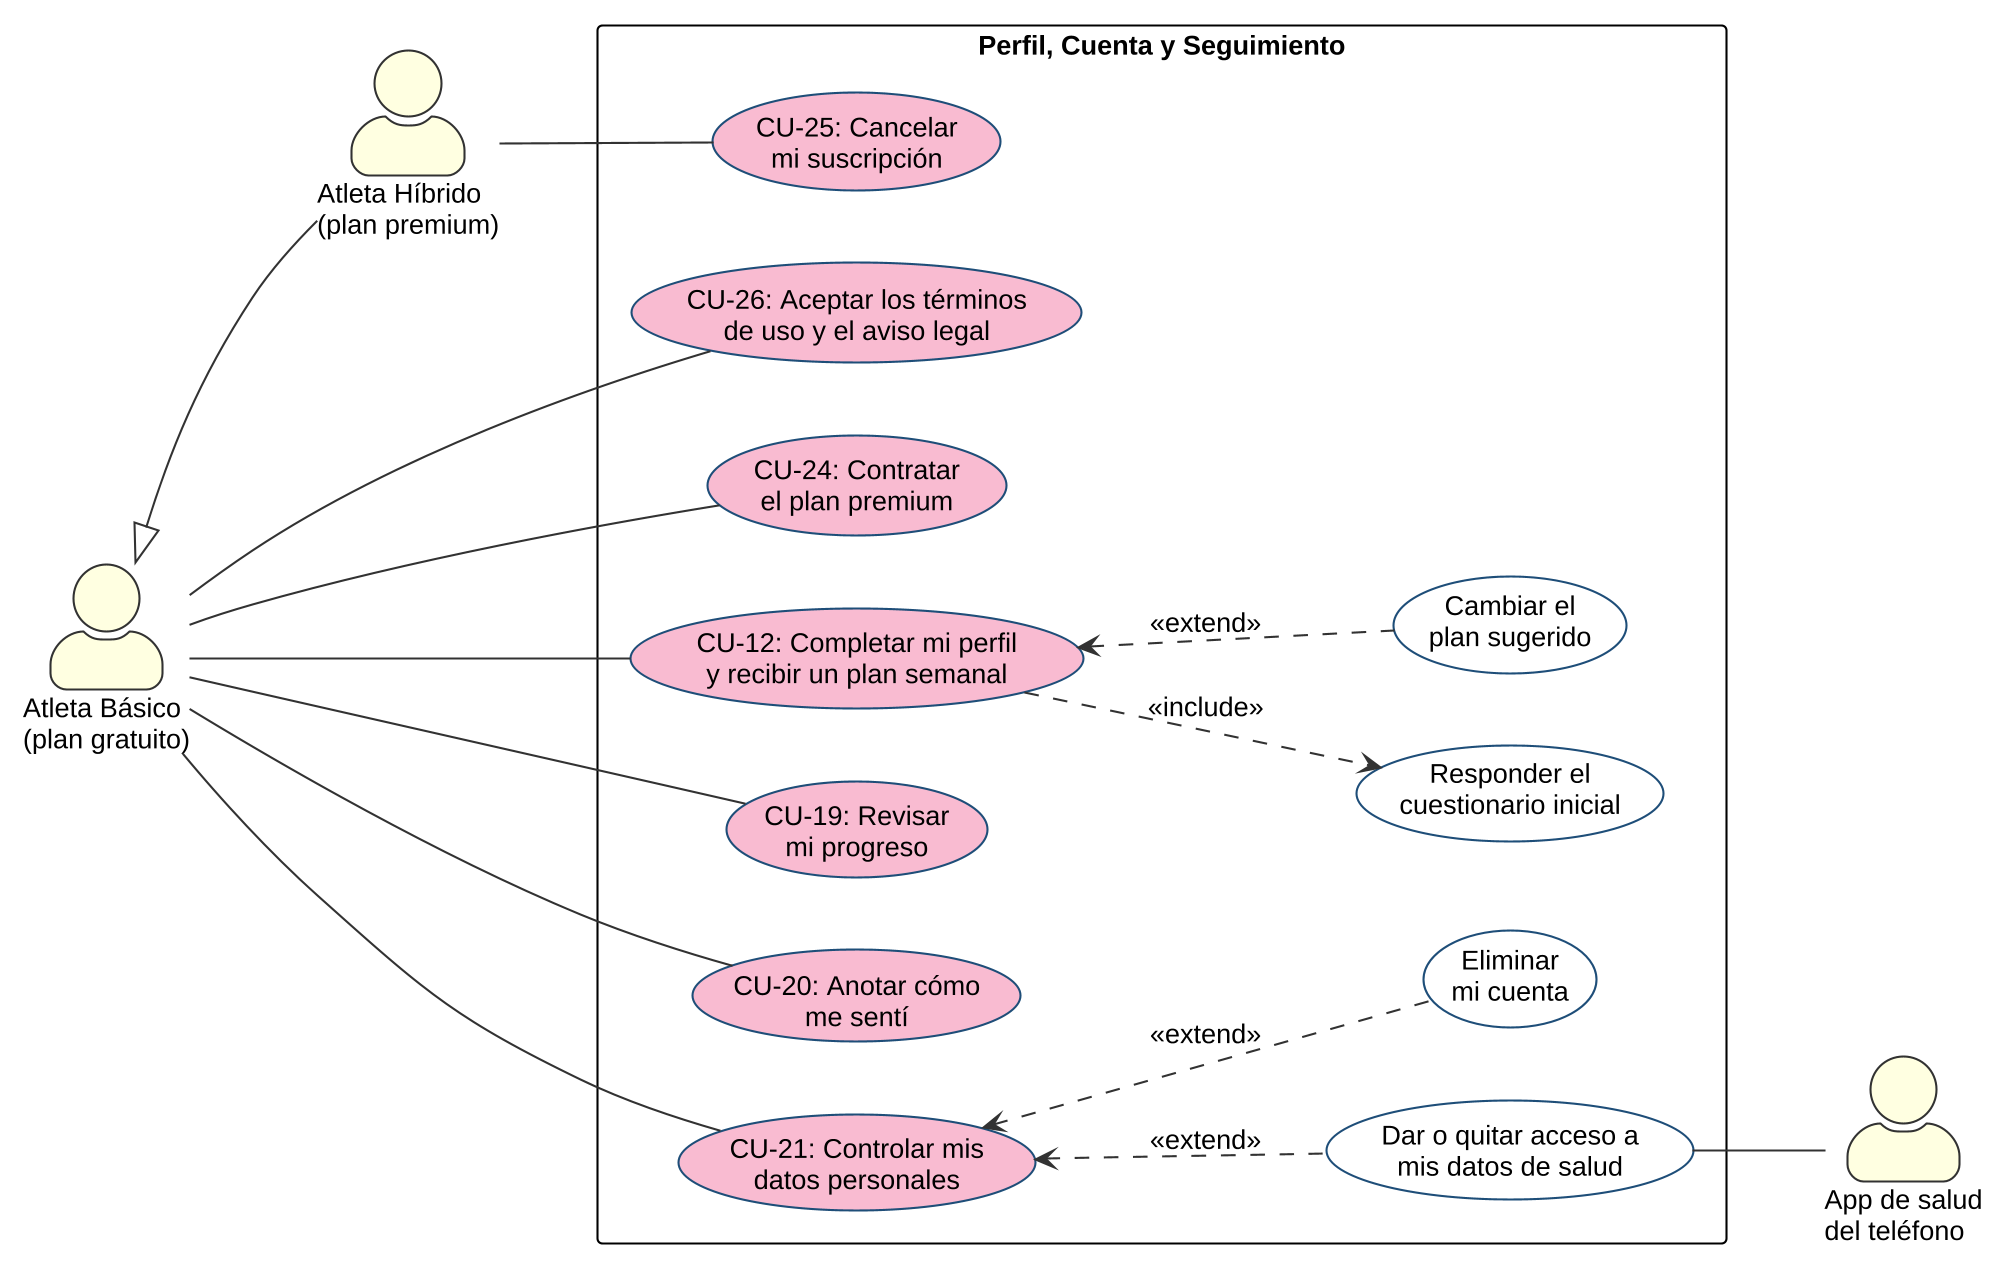
\includegraphics[width=0.9\textwidth]{figuras/casos_de_uso/cu_perfil.png}
    \caption{Diagrama de Casos de Uso: Perfil, Cuenta y Seguimiento.}
    \label{fig:cu_perfil}
\end{figure}

\begin{figure}[h!]
    \centering
    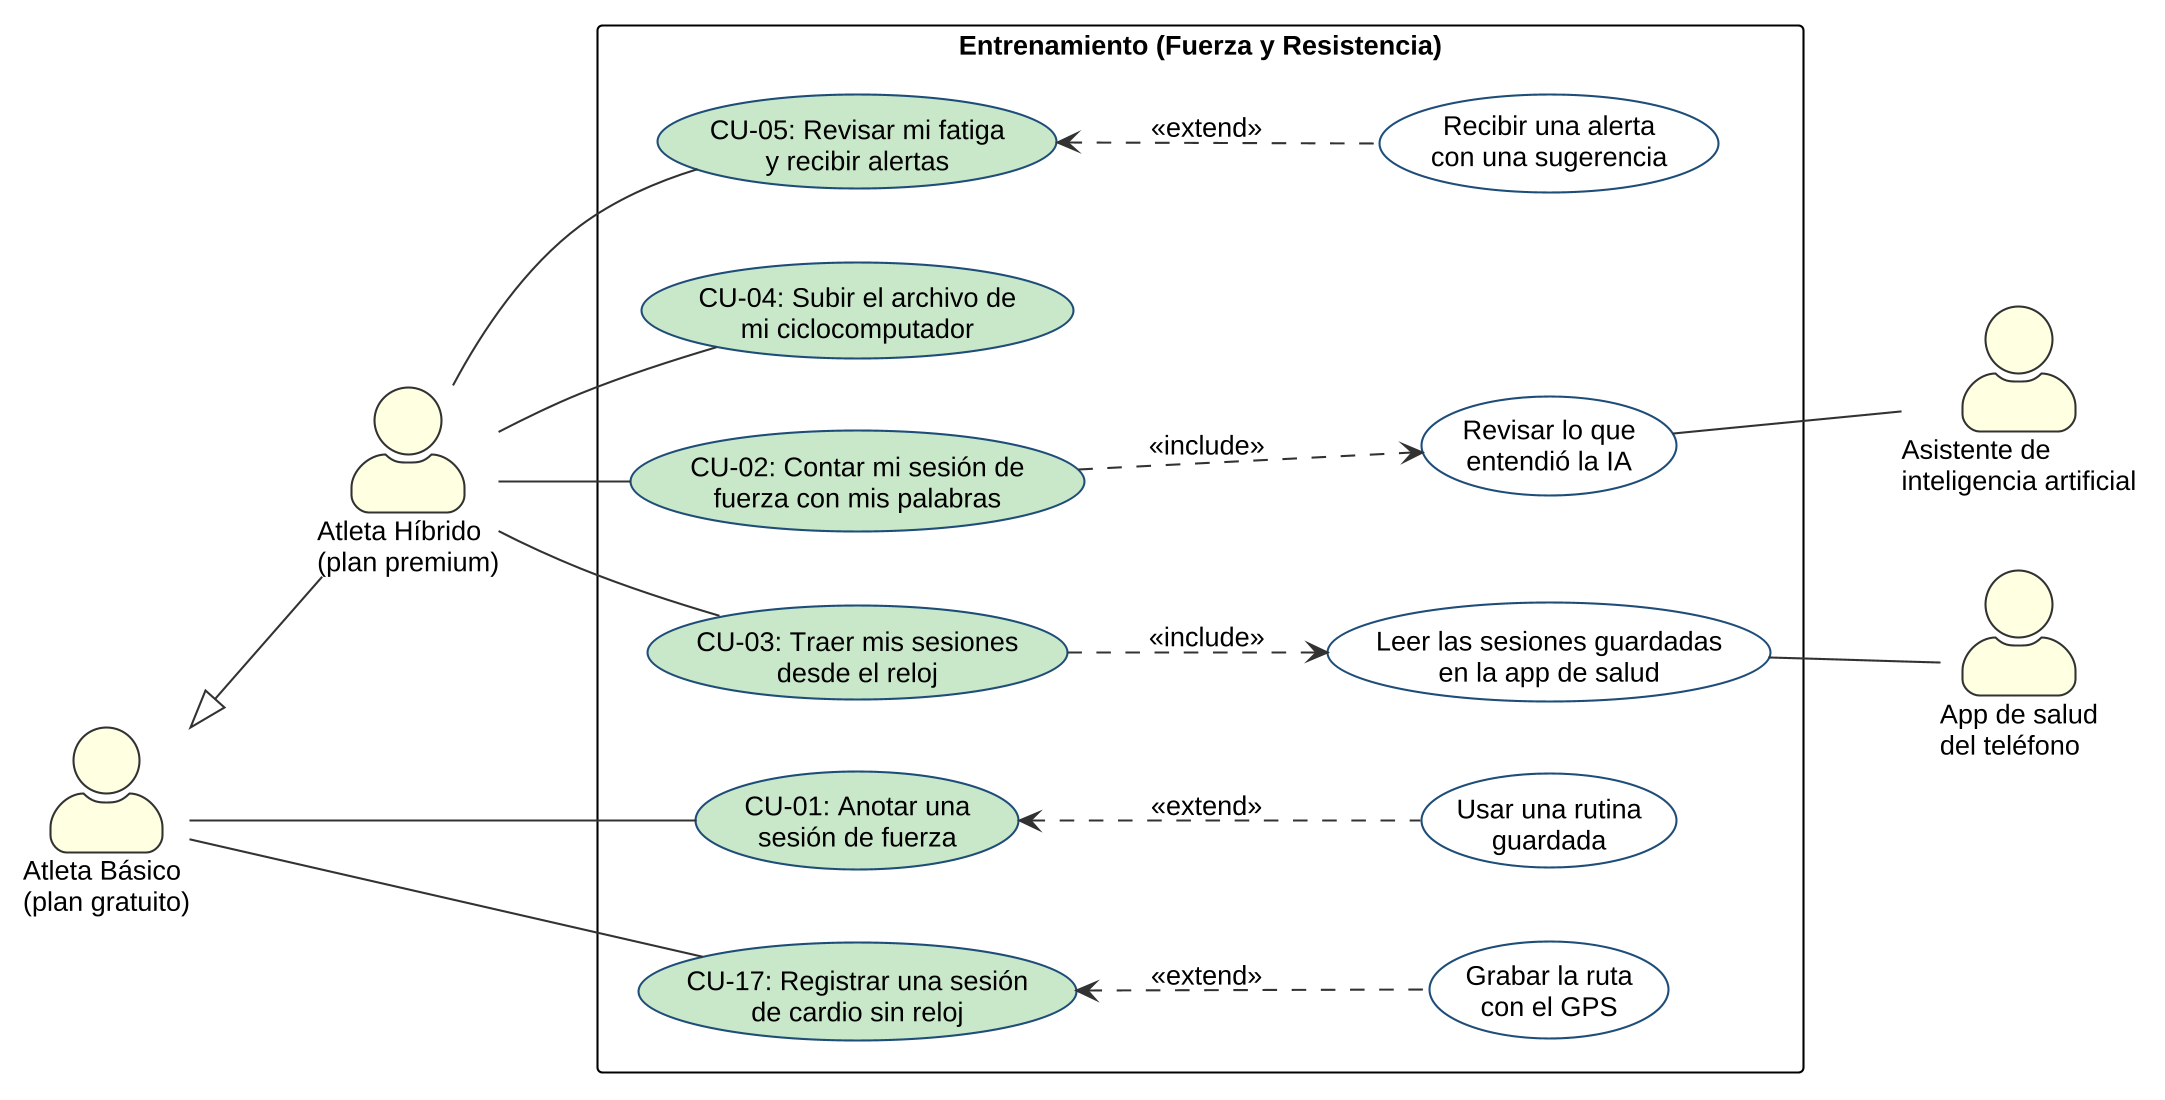
\includegraphics[width=0.95\textwidth]{figuras/casos_de_uso/cu_entrenamiento.png}
    \caption{Diagrama de Casos de Uso: Entrenamiento (Fuerza y Resistencia).}
    \label{fig:cu_entrenamiento}
\end{figure}
\begin{figure}[h!]
    \centering
    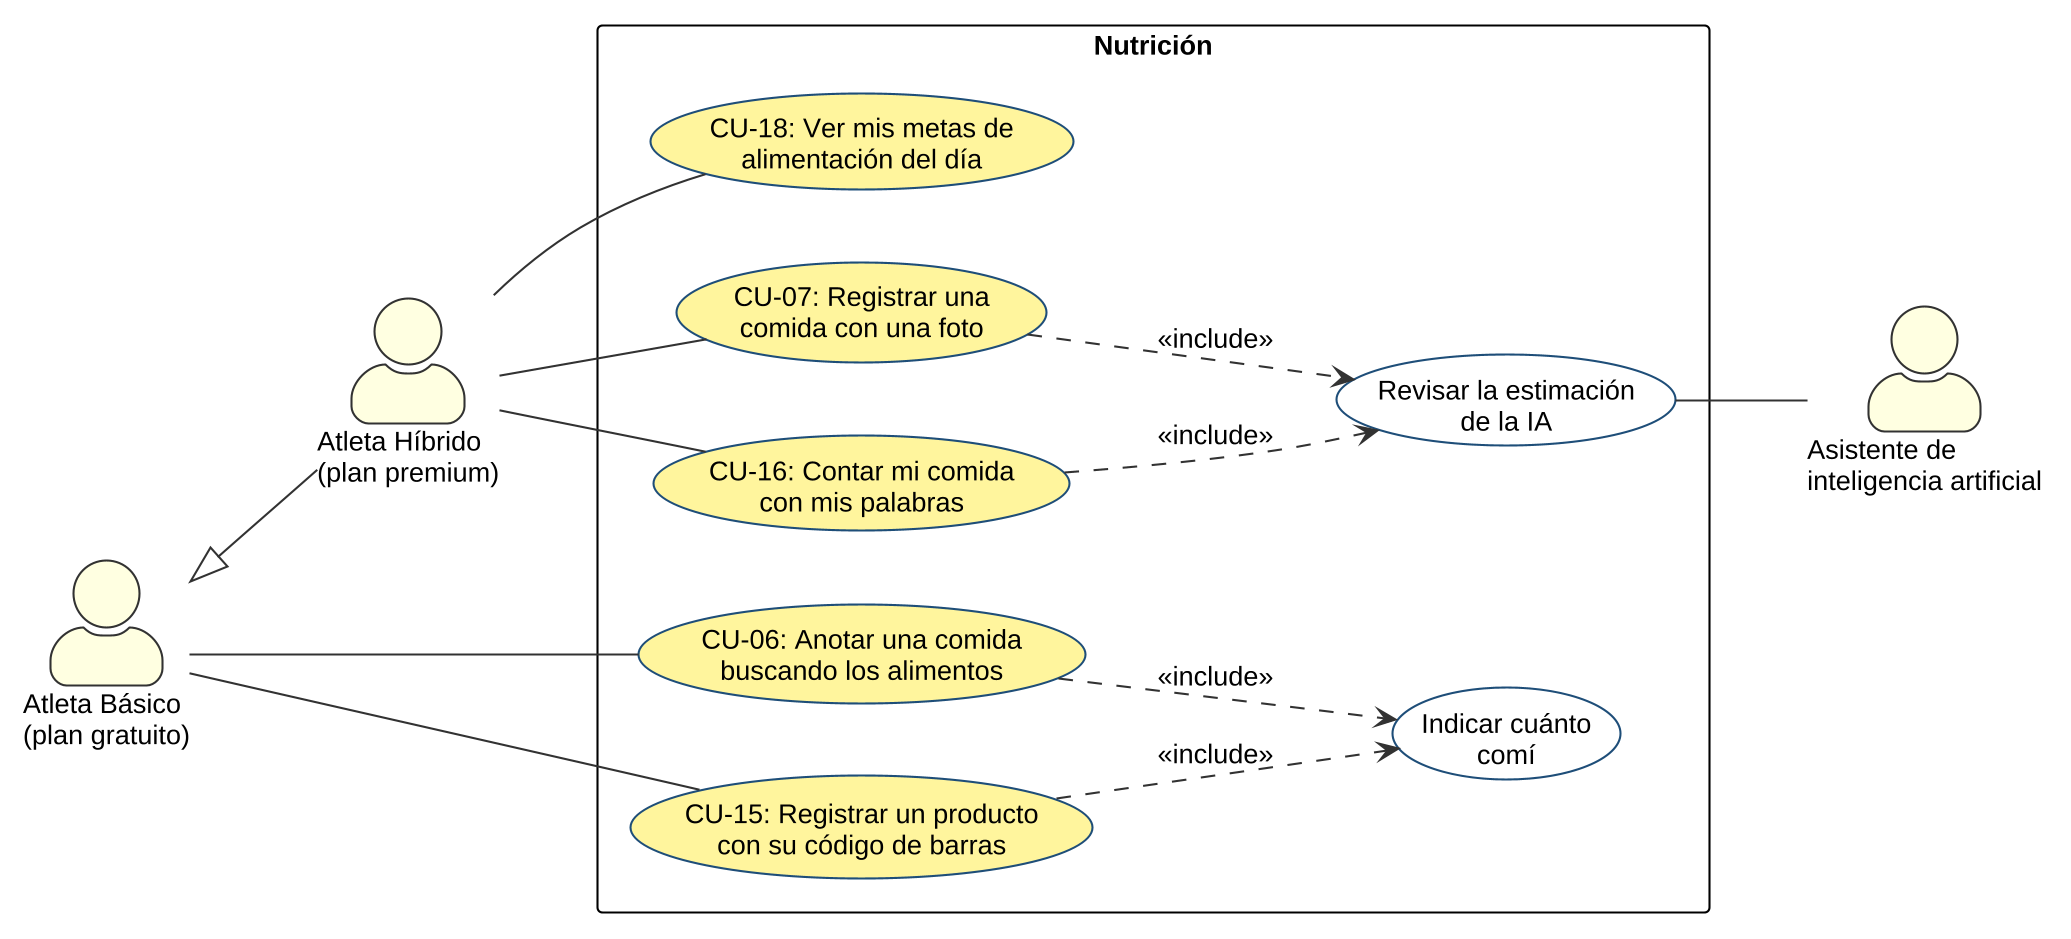
\includegraphics[width=0.95\textwidth]{figuras/casos_de_uso/cu_nutricion.png}
    \caption{Diagrama de Casos de Uso: Nutrición.}
    \label{fig:cu_nutricion}
\end{figure}

\begin{figure}[h!]
    \centering
    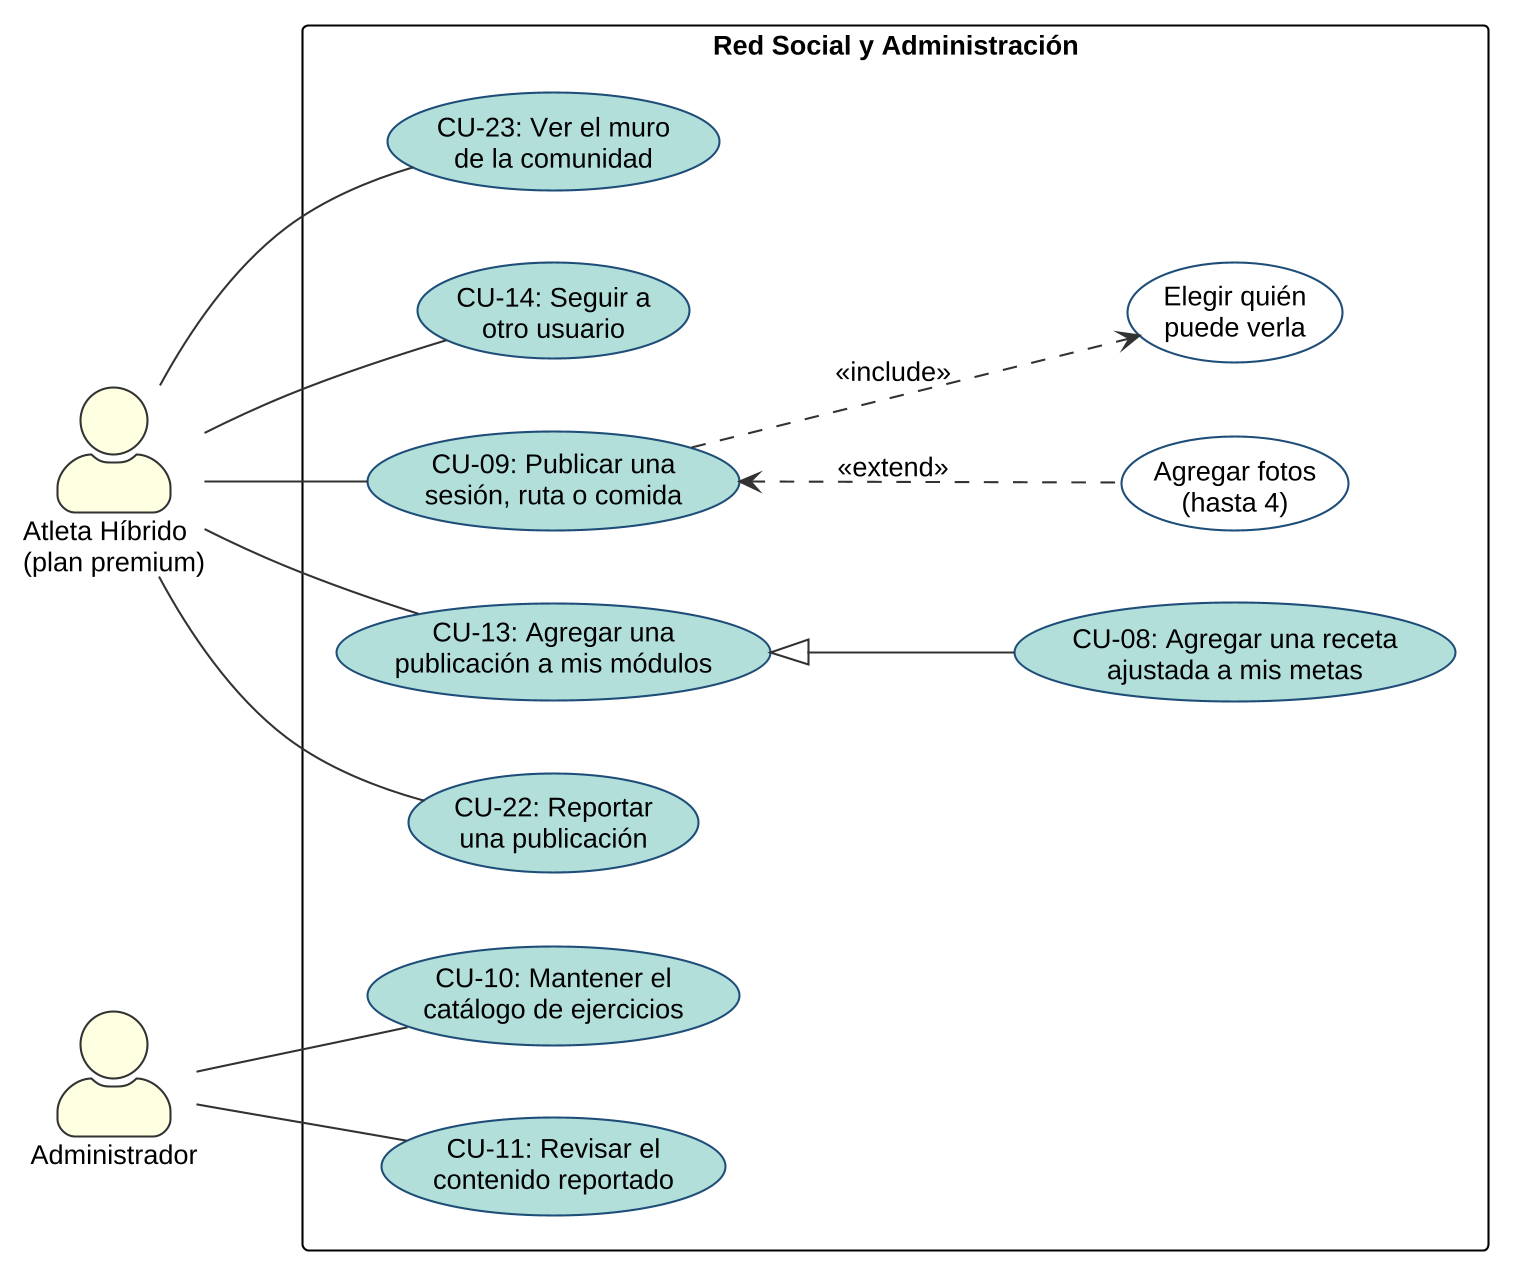
\includegraphics[width=0.85\textwidth]{figuras/casos_de_uso/cu_comunidad.png}
    \caption{Diagrama de Casos de Uso: Red Social y Administración.}
    \label{fig:cu_comunidad}
\end{figure}
\clearpage
\subsubsection{Descripción de Alto Nivel de Casos de Uso}
A continuación se describe cada caso de uso de los diagramas anteriores, con el requerimiento funcional al que responde. Su flujo normal y sus flujos alternativos se detallan en el Diseño Funcional del capítulo siguiente. Los casos CU-01 a CU-14 vienen de las versiones anteriores del documento, y los casos CU-15 a CU-26 se agregaron para que todos los requerimientos tengan al menos un caso de uso.

\noindent
\begin{tabular}{|p{3.5cm}|p{11.5cm}|}
    \hline
    \rowcolor[HTML]{EFEFEF}
    \textbf{Identificador} & \textbf{CU-01} \\ \hline
    \textbf{Nombre} & Anotar una sesión de fuerza \\ \hline
    \textbf{Actor Principal} & Atleta Básico / Atleta Híbrido \\ \hline
    \textbf{Descripción} & El usuario elige los ejercicios que hizo, desde la lista de ejercicios o desde una rutina que guardó antes, y anota las series, las repeticiones, el peso y qué tan duro lo sintió. La aplicación guarda la sesión y la suma a su historial. \\ \hline
    \textbf{RF Asociados} & R01 \\ \hline
\end{tabular}
\vspace{0.5cm}

\noindent
\begin{tabular}{|p{3.5cm}|p{11.5cm}|}
    \hline
    \rowcolor[HTML]{EFEFEF}
    \textbf{Identificador} & \textbf{CU-02} \\ \hline
    \textbf{Nombre} & Contar mi sesión de fuerza con mis palabras \\ \hline
    \textbf{Actor Principal} & Atleta Híbrido \\ \hline
    \textbf{Actores Secundarios} & Asistente de inteligencia artificial \\ \hline
    \textbf{Descripción} & El usuario escribe o dicta lo que hizo, por ejemplo ``sentadilla, 4 series de 8 con 80 kilos''. La aplicación lo ordena en ejercicios, series y pesos, y se lo muestra para que lo revise. El usuario corrige lo que haga falta y lo guarda. \\ \hline
    \textbf{RF Asociados} & R01 \\ \hline
\end{tabular}
\vspace{0.5cm}
\newpage
\noindent
\begin{tabular}{|p{3.5cm}|p{11.5cm}|}
    \hline
    \rowcolor[HTML]{EFEFEF}
    \textbf{Identificador} & \textbf{CU-03} \\ \hline
    \textbf{Nombre} & Traer mis sesiones desde el reloj \\ \hline
    \textbf{Actor Principal} & Atleta Híbrido \\ \hline
    \textbf{Actores Secundarios} & App de salud del teléfono \\ \hline
    \textbf{Descripción} & Después de entrenar con su reloj, la aplicación trae sola las sesiones nuevas de ciclismo, running o trekking desde la app de salud del teléfono, con su duración, su distancia y su pulso. Así no tiene que anotar nada a mano. La primera vez, la aplicación le pide permiso para leer esos datos. \\ \hline
    \textbf{RF Asociados} & R02 \\ \hline
\end{tabular}
\vspace{0.5cm}

\noindent
\begin{tabular}{|p{3.5cm}|p{11.5cm}|}
    \hline
    \rowcolor[HTML]{EFEFEF}
    \textbf{Identificador} & \textbf{CU-04} \\ \hline
    \textbf{Nombre} & Subir el archivo de mi ciclocomputador \\ \hline
    \textbf{Actor Principal} & Atleta Híbrido \\ \hline
    \textbf{Descripción} & El usuario sube el archivo que exportó desde su ciclocomputador o reloj. La aplicación lo lee y le muestra la sesión con todo detalle, como la potencia, la cadencia y el pulso a lo largo de la salida. \\ \hline
    \textbf{RF Asociados} & R02 \\ \hline
\end{tabular}
\vspace{0.5cm}

\noindent
\begin{tabular}{|p{3.5cm}|p{11.5cm}|}
    \hline
    \rowcolor[HTML]{EFEFEF}
    \textbf{Identificador} & \textbf{CU-05} \\ \hline
    \textbf{Nombre} & Revisar mi fatiga y recibir alertas \\ \hline
    \textbf{Actor Principal} & Atleta Híbrido \\ \hline
    \textbf{Descripción} & El usuario ve en un resumen cuánto se ha cargado en la semana, sumando la fuerza y el cardio. Si la aplicación nota que viene muy cansado y tiene un entrenamiento exigente al día siguiente, le manda un aviso con una sugerencia, por ejemplo bajar el peso o mover la sesión. También le avisa si dejó poco tiempo entre una sesión de fuerza y una de cardio. El usuario decide si la sigue. \\ \hline
    \textbf{RF Asociados} & R03 \\ \hline
\end{tabular}
\vspace{0.5cm}
\newpage
\noindent
\begin{tabular}{|p{3.5cm}|p{11.5cm}|}
    \hline
    \rowcolor[HTML]{EFEFEF}
    \textbf{Identificador} & \textbf{CU-06} \\ \hline
    \textbf{Nombre} & Anotar una comida buscando los alimentos \\ \hline
    \textbf{Actor Principal} & Atleta Básico / Atleta Híbrido \\ \hline
    \textbf{Descripción} & El usuario busca lo que comió en la lista de alimentos, indica cuánto comió y lo guarda en su diario del día. La aplicación le muestra las calorías y los macronutrientes de la comida y cuánto lleva en el día. \\ \hline
    \textbf{RF Asociados} & R04 \\ \hline
\end{tabular}
\vspace{0.5cm}

\noindent
\begin{tabular}{|p{3.5cm}|p{11.5cm}|}
    \hline
    \rowcolor[HTML]{EFEFEF}
    \textbf{Identificador} & \textbf{CU-07} \\ \hline
    \textbf{Nombre} & Registrar una comida con una foto \\ \hline
    \textbf{Actor Principal} & Atleta Híbrido \\ \hline
    \textbf{Actores Secundarios} & Asistente de inteligencia artificial \\ \hline
    \textbf{Descripción} & El usuario le saca una foto a su plato. La aplicación estima qué alimentos hay, en qué cantidad y cuántas calorías y macronutrientes tienen. El usuario revisa la estimación, la corrige si hace falta y la guarda. Cuando la aplicación no está segura del resultado, se lo avisa para que lo revise con más cuidado. La foto no se guarda, salvo que el usuario la quiera publicar. \\ \hline
    \textbf{RF Asociados} & R04 \\ \hline
\end{tabular}
\vspace{0.5cm}

\noindent
\begin{tabular}{|p{3.5cm}|p{11.5cm}|}
    \hline
    \rowcolor[HTML]{EFEFEF}
    \textbf{Identificador} & \textbf{CU-08} \\ \hline
    \textbf{Nombre} & Agregar una receta ajustada a mis metas \\ \hline
    \textbf{Actor Principal} & Atleta Híbrido \\ \hline
    \textbf{Descripción} & El usuario ve una receta en el muro y la agrega a su módulo de nutrición. La aplicación ajusta la cantidad de cada ingrediente según lo que le falta comer ese día, manteniendo las proporciones de la receta original. Es un caso particular de CU-13. \\ \hline
    \textbf{RF Asociados} & R12 \\ \hline
\end{tabular}
\vspace{0.5cm}
\newpage
\noindent
\begin{tabular}{|p{3.5cm}|p{11.5cm}|}
    \hline
    \rowcolor[HTML]{EFEFEF}
    \textbf{Identificador} & \textbf{CU-09} \\ \hline
    \textbf{Nombre} & Publicar una sesión, ruta o comida \\ \hline
    \textbf{Actor Principal} & Atleta Híbrido \\ \hline
    \textbf{Descripción} & El usuario elige una sesión de fuerza, una ruta o una comida que ya registró, le agrega un texto y, si quiere, hasta 4 fotos, declarando que son suyas o que tiene permiso para publicarlas. Luego elige quién la puede ver (todos, sus seguidores o solo él). Si publica una ruta, la aplicación oculta el inicio y el final del recorrido para que no se sepa dónde vive. \\ \hline
    \textbf{RF Asociados} & R08 \\ \hline
\end{tabular}
\vspace{0.5cm}

\noindent
\begin{tabular}{|p{3.5cm}|p{11.5cm}|}
    \hline
    \rowcolor[HTML]{EFEFEF}
    \textbf{Identificador} & \textbf{CU-10} \\ \hline
    \textbf{Nombre} & Mantener el catálogo de ejercicios \\ \hline
    \textbf{Actor Principal} & Administrador \\ \hline
    \textbf{Descripción} & El administrador agrega, cambia o desactiva ejercicios de la lista que usan los atletas, indicando qué músculos trabajan y qué equipamiento necesitan. La aplicación le avisa si el ejercicio ya existe. \\ \hline
    \textbf{RF Asociados} & R11 \\ \hline
\end{tabular}
\vspace{0.5cm}

\noindent
\begin{tabular}{|p{3.5cm}|p{11.5cm}|}
    \hline
    \rowcolor[HTML]{EFEFEF}
    \textbf{Identificador} & \textbf{CU-11} \\ \hline
    \textbf{Nombre} & Revisar el contenido reportado \\ \hline
    \textbf{Actor Principal} & Administrador \\ \hline
    \textbf{Descripción} & El administrador revisa las publicaciones, fotos y recetas que reportaron los usuarios. Si no cumplen las normas de la comunidad o pueden ser peligrosas para la salud, las oculta. La aplicación guarda quién tomó la decisión y por qué. \\ \hline
    \textbf{RF Asociados} & R11 \\ \hline
\end{tabular}
\vspace{0.5cm}
\newpage
\noindent
\begin{tabular}{|p{3.5cm}|p{11.5cm}|}
    \hline
    \rowcolor[HTML]{EFEFEF}
    \textbf{Identificador} & \textbf{CU-12} \\ \hline
    \textbf{Nombre} & Completar mi perfil y recibir un plan semanal \\ \hline
    \textbf{Actor Principal} & Atleta Básico / Atleta Híbrido \\ \hline
    \textbf{Descripción} & Al crear su cuenta, el usuario responde preguntas sobre su experiencia, sus objetivos, los días que puede entrenar, su equipamiento, los deportes que practica, su edad, su sexo, su estatura y su peso. Con eso, la aplicación le sugiere un plan para la semana, que puede aceptar, cambiar o ignorar. Cada semana el plan se ajusta según lo que el usuario cumplió y cómo se sintió. \\ \hline
    \textbf{RF Asociados} & R13 \\ \hline
\end{tabular}
\vspace{0.5cm}

\noindent
\begin{tabular}{|p{3.5cm}|p{11.5cm}|}
    \hline
    \rowcolor[HTML]{EFEFEF}
    \textbf{Identificador} & \textbf{CU-13} \\ \hline
    \textbf{Nombre} & Agregar una publicación a mis módulos \\ \hline
    \textbf{Actor Principal} & Atleta Híbrido \\ \hline
    \textbf{Descripción} & El usuario ve en el muro una publicación de otra persona, por ejemplo una rutina de pecho, y pulsa ``Agregar a mis rutinas''. La rutina queda guardada como suya, indicando quién la creó. Si es una ruta, queda en su módulo de cardio, y si es una receta, en su módulo de nutrición (CU-08). \\ \hline
    \textbf{RF Asociados} & R12 \\ \hline
\end{tabular}
\vspace{0.5cm}

\noindent
\begin{tabular}{|p{3.5cm}|p{11.5cm}|}
    \hline
    \rowcolor[HTML]{EFEFEF}
    \textbf{Identificador} & \textbf{CU-14} \\ \hline
    \textbf{Nombre} & Seguir a otro usuario \\ \hline
    \textbf{Actor Principal} & Atleta Híbrido \\ \hline
    \textbf{Descripción} & El usuario encuentra a otra persona en el muro o en el buscador y la sigue. Desde ese momento ve las publicaciones de esa persona en su muro. Puede dejar de seguirla cuando quiera. \\ \hline
    \textbf{RF Asociados} & R08 \\ \hline
\end{tabular}
\vspace{0.5cm}
\newpage
\noindent
\begin{tabular}{|p{3.5cm}|p{11.5cm}|}
    \hline
    \rowcolor[HTML]{EFEFEF}
    \textbf{Identificador} & \textbf{CU-15} \\ \hline
    \textbf{Nombre} & Registrar un producto con su código de barras \\ \hline
    \textbf{Actor Principal} & Atleta Básico / Atleta Híbrido \\ \hline
    \textbf{Descripción} & El usuario escanea con la cámara el código de barras de un producto envasado. La aplicación le muestra sus calorías y macronutrientes. El usuario indica cuánto comió y lo guarda. \\ \hline
    \textbf{RF Asociados} & R04 \\ \hline
\end{tabular}
\vspace{0.5cm}

\noindent
\begin{tabular}{|p{3.5cm}|p{11.5cm}|}
    \hline
    \rowcolor[HTML]{EFEFEF}
    \textbf{Identificador} & \textbf{CU-16} \\ \hline
    \textbf{Nombre} & Contar mi comida con mis palabras \\ \hline
    \textbf{Actor Principal} & Atleta Híbrido \\ \hline
    \textbf{Actores Secundarios} & Asistente de inteligencia artificial \\ \hline
    \textbf{Descripción} & El usuario escribe o dicta lo que comió, por ejemplo ``un plato de arroz con pollo y una ensalada''. La aplicación estima los alimentos, las cantidades y los macronutrientes. El usuario revisa la estimación, la corrige si hace falta y la guarda. \\ \hline
    \textbf{RF Asociados} & R04 \\ \hline
\end{tabular}
\vspace{0.5cm}

\noindent
\begin{tabular}{|p{3.5cm}|p{11.5cm}|}
    \hline
    \rowcolor[HTML]{EFEFEF}
    \textbf{Identificador} & \textbf{CU-17} \\ \hline
    \textbf{Nombre} & Registrar una sesión de cardio sin reloj \\ \hline
    \textbf{Actor Principal} & Atleta Básico / Atleta Híbrido \\ \hline
    \textbf{Descripción} & El usuario graba su salida de ciclismo, running o trekking con el GPS del teléfono, o la anota a mano con su duración, su distancia y qué tan duro la sintió. La aplicación la guarda y la considera en su carga de la semana. \\ \hline
    \textbf{RF Asociados} & R02 \\ \hline
\end{tabular}
\vspace{0.5cm}
\newpage
\noindent
\begin{tabular}{|p{3.5cm}|p{11.5cm}|}
    \hline
    \rowcolor[HTML]{EFEFEF}
    \textbf{Identificador} & \textbf{CU-18} \\ \hline
    \textbf{Nombre} & Ver mis metas de alimentación del día \\ \hline
    \textbf{Actor Principal} & Atleta Híbrido \\ \hline
    \textbf{Descripción} & El usuario abre su resumen de nutrición y ve cuántas calorías y macronutrientes le conviene comer ese día, según lo que entrenó o tiene planificado, y cuánto le falta. También le sugiere en qué momento conviene comer. Son sugerencias y no una dieta. \\ \hline
    \textbf{RF Asociados} & R05 \\ \hline
\end{tabular}
\vspace{0.5cm}

\noindent
\begin{tabular}{|p{3.5cm}|p{11.5cm}|}
    \hline
    \rowcolor[HTML]{EFEFEF}
    \textbf{Identificador} & \textbf{CU-19} \\ \hline
    \textbf{Nombre} & Revisar mi progreso \\ \hline
    \textbf{Actor Principal} & Atleta Básico / Atleta Híbrido \\ \hline
    \textbf{Descripción} & El usuario abre su historial y elige ver un día o un mes. La aplicación le muestra juntos sus entrenamientos, sus comidas y cómo ha cambiado su carga en el tiempo. \\ \hline
    \textbf{RF Asociados} & R06 \\ \hline
\end{tabular}
\vspace{0.5cm}

\noindent
\begin{tabular}{|p{3.5cm}|p{11.5cm}|}
    \hline
    \rowcolor[HTML]{EFEFEF}
    \textbf{Identificador} & \textbf{CU-20} \\ \hline
    \textbf{Nombre} & Anotar cómo me sentí \\ \hline
    \textbf{Actor Principal} & Atleta Básico / Atleta Híbrido \\ \hline
    \textbf{Descripción} & Después de un entrenamiento o de una comida, el usuario escribe cómo se sintió, por ejemplo si tuvo alguna molestia o si la comida le cayó pesada. La nota queda junto a ese registro para revisarla después. \\ \hline
    \textbf{RF Asociados} & R07 \\ \hline
\end{tabular}
\vspace{0.5cm}
\newpage
\noindent
\begin{tabular}{|p{3.5cm}|p{11.5cm}|}
    \hline
    \rowcolor[HTML]{EFEFEF}
    \textbf{Identificador} & \textbf{CU-21} \\ \hline
    \textbf{Nombre} & Controlar mis datos personales \\ \hline
    \textbf{Actor Principal} & Atleta Básico / Atleta Híbrido \\ \hline
    \textbf{Actores Secundarios} & App de salud del teléfono \\ \hline
    \textbf{Descripción} & El usuario decide si la aplicación puede leer sus datos de salud y puede cambiar esa decisión cuando quiera. También puede revisar y corregir sus datos o eliminar su cuenta. Si elimina la cuenta, se borran todos sus datos. \\ \hline
    \textbf{RF Asociados} & R09 \\ \hline
\end{tabular}
\vspace{0.5cm}

\noindent
\begin{tabular}{|p{3.5cm}|p{11.5cm}|}
    \hline
    \rowcolor[HTML]{EFEFEF}
    \textbf{Identificador} & \textbf{CU-22} \\ \hline
    \textbf{Nombre} & Reportar una publicación \\ \hline
    \textbf{Actor Principal} & Atleta Híbrido \\ \hline
    \textbf{Descripción} & El usuario reporta una publicación o una foto que le parece inapropiada o peligrosa y elige el motivo. El administrador la revisa después (CU-11). \\ \hline
    \textbf{RF Asociados} & R08, R11 \\ \hline
\end{tabular}
\vspace{0.5cm}

\noindent
\begin{tabular}{|p{3.5cm}|p{11.5cm}|}
    \hline
    \rowcolor[HTML]{EFEFEF}
    \textbf{Identificador} & \textbf{CU-23} \\ \hline
    \textbf{Nombre} & Ver el muro de la comunidad \\ \hline
    \textbf{Actor Principal} & Atleta Híbrido \\ \hline
    \textbf{Descripción} & El usuario abre el muro y ve las publicaciones más recientes de las personas que sigue, con sus fotos. Desde ahí puede abrir una publicación, agregarla a sus módulos (CU-13) o reportarla (CU-22). \\ \hline
    \textbf{RF Asociados} & R08 \\ \hline
\end{tabular}
\vspace{0.5cm}

\noindent
\begin{tabular}{|p{3.5cm}|p{11.5cm}|}
    \hline
    \rowcolor[HTML]{EFEFEF}
    \textbf{Identificador} & \textbf{CU-24} \\ \hline
    \textbf{Nombre} & Contratar el plan premium \\ \hline
    \textbf{Actor Principal} & Atleta Básico \\ \hline
    \textbf{Descripción} & El usuario ve qué incluye el plan premium, cuánto cuesta en total y cada cuánto se cobra. Si le interesa, lo contrata y desde ese momento tiene todas sus funciones. \\ \hline
    \textbf{RF Asociados} & R14 \\ \hline
\end{tabular}
\vspace{0.5cm}

\noindent
\begin{tabular}{|p{3.5cm}|p{11.5cm}|}
    \hline
    \rowcolor[HTML]{EFEFEF}
    \textbf{Identificador} & \textbf{CU-25} \\ \hline
    \textbf{Nombre} & Cancelar mi suscripción \\ \hline
    \textbf{Actor Principal} & Atleta Híbrido \\ \hline
    \textbf{Descripción} & El usuario cancela su suscripción desde la aplicación, que lo lleva a la pantalla de suscripciones de su tienda, donde confirma la cancelación. Sigue con el plan premium hasta que termine el periodo pagado, y después vuelve al plan gratuito conservando sus datos. \\ \hline
    \textbf{RF Asociados} & R14 \\ \hline
\end{tabular}
\vspace{0.5cm}

\noindent
\begin{tabular}{|p{3.5cm}|p{11.5cm}|}
    \hline
    \rowcolor[HTML]{EFEFEF}
    \textbf{Identificador} & \textbf{CU-26} \\ \hline
    \textbf{Nombre} & Aceptar los términos de uso y el aviso legal \\ \hline
    \textbf{Actor Principal} & Atleta Básico / Atleta Híbrido \\ \hline
    \textbf{Descripción} & Al crear su cuenta, el usuario lee los términos de uso y el aviso legal, y los acepta para poder seguir. Si los términos cambian más adelante, la aplicación se los vuelve a mostrar. \\ \hline
    \textbf{RF Asociados} & R15 \\ \hline
\end{tabular}
\vspace{0.5cm}
\newpage
\begin{table}[h!]
    \centering
    \renewcommand{\arraystretch}{1.3}
    \begin{tabular}{|p{1.5cm}|>{\raggedright\arraybackslash}p{7cm}|>{\raggedright\arraybackslash}p{6cm}|}
        \hline
        \rowcolor[HTML]{EFEFEF}
        \textbf{ID} & \textbf{Requerimiento} & \textbf{Casos de uso} \\ \hline
        R01 & Registro de entrenamientos de fuerza & CU-01, CU-02 \\ \hline
        R02 & Registro de entrenamientos de resistencia & CU-03, CU-04, CU-17 \\ \hline
        R03 & Alertas de fatiga y ajuste del entrenamiento & CU-05 \\ \hline
        R04 & Registro de comidas & CU-06, CU-07, CU-15, CU-16 \\ \hline
        R05 & Metas de alimentación según el entrenamiento & CU-18 \\ \hline
        R06 & Seguimiento del progreso & CU-19 \\ \hline
        R07 & Registro de sensaciones & CU-20 \\ \hline
        R08 & Red social deportiva & CU-09, CU-14, CU-22, CU-23 \\ \hline
        R09 & Control de datos personales & CU-21 \\ \hline
        R10 & Uso simple y rápido & Se cubre en todos los casos de uso y con los requisitos no funcionales. \\ \hline
        R11 & Administración de la plataforma & CU-10, CU-11, CU-22 \\ \hline
        R12 & Agregar contenido de la comunidad a mis módulos & CU-08, CU-13 \\ \hline
        R13 & Perfil del usuario y plan sugerido & CU-12 \\ \hline
        R14 & Suscripción al plan premium & CU-24, CU-25 \\ \hline
        R15 & Términos de uso y aviso legal & CU-09, CU-26 \\ \hline
    \end{tabular}
    \caption{Relación entre los requerimientos funcionales y los casos de uso.}
    \label{tab:cu_requerimientos}
\end{table}
\newpage
\subsection{Comentarios Generales del Capítulo}
En este capítulo se ha consolidado el puente entre la visión de negocio y la implementación técnica de la plataforma. El capítulo partió con un Modelo de Negocios de cinco procesos, que son el registro de cardio con el cálculo de fatiga, el registro de comidas con sus metas, la publicación y el uso de contenido de la comunidad, el registro de fuerza y el plan sugerido. Posteriormente, la trazabilidad de los requerimientos garantizó que cada especificación funcional y no funcional del software nazca directamente de una necesidad operativa comprobada, mitigando el riesgo de desarrollar funcionalidades superfluas. 

Además, se incorporaron requerimientos centrados en la personalización, como el perfil del usuario con su plan sugerido, y en la red social deportiva, donde el contenido que publican otros usuarios se puede agregar directamente a los propios módulos.
\\\\
Finalmente, la especificación de los Casos de Uso, apoyada por sus respectivos diagramas e identificación de actores primarios y secundarios, delimitó con exactitud la frontera del sistema. Con este sólido marco de requerimientos finalizado, alineado a las restricciones normativas chilenas y a las dependencias de hardware de terceros, el proyecto cuenta con las bases necesarias para transicionar hacia la fase de Ingeniería de Diseño, donde se definirá la arquitectura de software detallada, el modelo de datos orientado a documentos y las interfaces de usuario.\newpage
\newpage
